\documentclass[twoside,notitlepage,11pt]{report}
%\usepackage{a4paper}
\usepackage{graphicx}
\usepackage{psfrag}
\usepackage{amsfonts}
\usepackage{amsbsy}
\usepackage{verbatimfile}
\usepackage{fancyhdr}
\usepackage{pstricks,pst-node}
% The next rawfonts package one is used in the ``datablad''.
\usepackage[only,egtrm]{rawfonts}
% Handle sorting in reference list
\usepackage{citesort}
% Create an index table
\usepackage{makeidx}

\newcommand{\smallverbatimfile}[1]{{\footnotesize\verbatimfile{#1}}}
\newcommand{\component}[5]{\begin{tabular}{|ll|}\hline {\bf Name:} & #1 \\ \hline {\bf Author:} & #2 \\ \hline {\bf Input parameters} & #3 \\ \hline {\bf Optional parameters} & #4 \\ \hline {\bf Notes} & #5 \\ \hline \end{tabular} \\ \noindent }

\def\reportnum{Ris{\o}--R--1xyz(EN)}

%\oddsidemargin 0cm
%\evensidemargin 0cm
\addtolength{\hoffset}{-1.4cm}
\topmargin 0cm
\textwidth 15cm
\textheight 22cm
\addtolength{\footskip}{1.6pt}
\addtolength{\headheight}{1.6pt}

\pagestyle{fancy}
\fancyhf{}
\fancyfoot[LE,RO]{\thepage}
\fancyfoot[LO,RE]{\reportnum}
\renewcommand{\headrulewidth}{0pt}
\renewcommand{\footrulewidth}{0pt}

\fancypagestyle{plain}{%
\fancyhf{}
\fancyfoot[LE,RO]{\thepage}
\fancyfoot[RE,LO]{\reportnum}
\renewcommand{\headrulewidth}{0pt}
\renewcommand{\footrulewidth}{0pt}}

\newcommand{\MCS}{{McStas}}
\newcommand{\version}{{1.9}}
\newcommand{\reldate}{{May 1st, 2005}}
\newcommand{\Ombold}{\mbox{\boldmath $\Omega$}}

% enable index generation
\makeindex

%\title{Component manual\\ to the neutron ray-tracing package
% \MCS ,\\ version \version}
%\author{Kim Lefmann and Peter Kj\ae r Willendrup \\
% Materials Research Department, \\
% Ris\o\ National Laboratory, 4000 Roskilde, Denmark;\\
% Emmanuel Farhi and Klaus Lieutenant \\ ILL, Grenoble, France}
%\date{\reldate \\[2\baselineskip]
%\begin{center}
%  \includegraphics[width=4.5in]{figures/vanadium-surf-2.eps}
%\end{center}
%
\includegraphics[width=0.45\myheight]{risoe-logo.eps}%
%}
\begin{document}

%\maketitle
% Emacs settings: -*-mode: latex; TeX-master: "manual.tex"; -*-

\begingroup                     % Make all definitions local.

%
% This was modified from risoe.sty, <2 Aug 95>
%
\catcode`\@=11
\def\@magscale#1{ scaled \magstep#1 }
\font\frtnbf = cmb10 \@magscale2
\font\twfvbf = cmbx10   \@magscale5 % extended bold
\def\maketitle{\par
 \begingroup
 \def\thefootnote{\fnsymbol{footnote}}
 \def\@makefnmark{\hbox to 0pt{$^{\@thefnmark}$\hss}}
 \if@twocolumn
 \twocolumn[\@maketitle]
 \else \newpage
 \global\@topnum\z@ \@maketitle \fi\thispagestyle{empty}\@thanks\newpage
 \endgroup
 \setcounter{footnote}{0}
 \let\maketitle\relax
 \let\@maketitle\relax
 \gdef\@thanks{}\gdef\@author{}\gdef\@title{}\let\thanks\relax}
\def\@maketitle{\newpage \baselineskip 30dd \mbox{}
 \marginpar{{\frtnbf \hfill \llap{\mbox{\reportnum \reportlan\qquad\qquad}}}}
 \par\noindent\mbox{
\includegraphics[height=1.5cm]{figures/risoe-logo.eps}\hspace{2mm}
\includegraphics[height=1.5cm]{figures/DTU_logo.ps}} \par
 \vskip 1.5cm
 {\twfvbf \noindent \@title \par} \vskip 20dd \baselineskip 16dd
 {\frtnbf\noindent\@author \par} 
 \vskip 0.5cm
 \begin{center}
     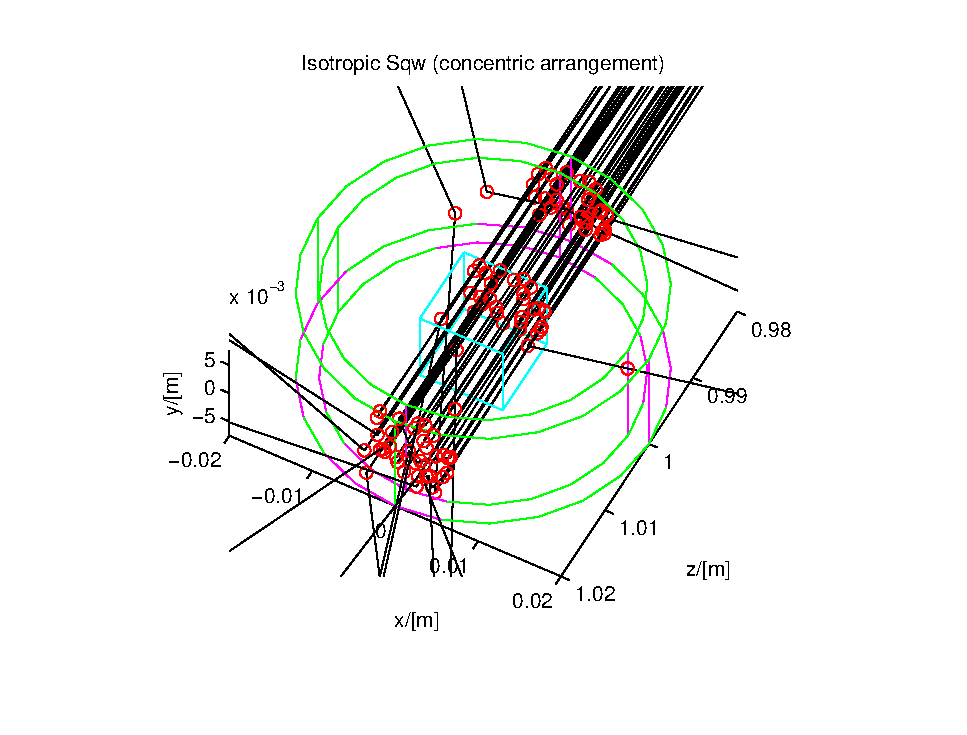
\includegraphics[width=\textwidth]{figures/sqw.eps}
   \end{center}
   \par \vfill \baselineskip 12dd
 \frtnbf\noindent Ris{\o} DTU, Roskilde, Denmark \par
 \vskip 4dd \noindent\ifcase\month\or
 January\or February\or March\or April\or May\or June\or
 July\or August\or September\or October\or November\or December\fi
 \space\number\year }

\let\reportlan=\relax
\def\month{5}                   % Released in November 2005
% Need to match front page line breaking.
\title{Component~Manual~for~\rlap{the}\\ % Avoid overfull message.
 X-Ray-Tracing~Package\\
 \MCX, Version \version\ }
\author{Peter Kj\ae r Willendrup, Erik Knudsen, Kim Lefmann and\\Emmanuel Farhi}
\maketitle
\endgroup


\thispagestyle{empty}
% Emacs settings: -*-mode: latex; TeX-master: "manual.tex"; -*-

\begin{abstract}
The software package McStas is a tool for carrying out Monte Carlo
ray-tracing simulations of neutron scattering instruments with high
complexity and precision. The simulations can compute most aspects of the
performance of instruments and samples
and can thus be used to optimize the use of existing equipment,
design new instrumentation, and carry out full virtual experiments.
McStas is based on a unique design where an automatic compilation process
translates high-level textual instrument descriptions into efficient
ANSI-C code. This design makes it simple to set up typical simulations
and also gives essentially unlimited freedom to handle more unusual
cases.

This report constitutes the component manual for McStas, and,
together with the manual for the McStas system, it
contains full documentation of all aspects of the program. It covers
a description of all official components of the \MCS\ package with
some theoretical background. Selected test
instruments and representative \MCS\ simulations performed with these
instruments are described in the User Manual.


\end{abstract}

\vskip\baselineskip\noindent
This report documents the components for McStas version \version,
released \reldate .
\vskip\baselineskip\noindent
The authors are:
\begin{quote}
\label{p:authors}
\vskip\baselineskip\noindent
Kim Lefmann \\
Materials Research Department, Ris{\o} National Laboratory, Roskilde, Denmark \\
email: \verb+kim.lefmann@risoe.dk+
\vskip\baselineskip\noindent
Peter Kj\ae r Willendrup \\
Materials Research Department, Ris{\o} National Laboratory, Roskilde, Denmark \\
email: \verb+peter.willendrup@risoe.dk+
\vskip\baselineskip\noindent
Kristian Nielsen \\
email: \verb+kristian.nielsen@mail.tele.dk+
\vskip\baselineskip\noindent
Emmanuel Farhi \\
Institut Laue-Langevin, Grenoble, France \\
email: \verb+farhi@ill.fr+
\vskip\baselineskip\noindent
Klaus Lieutenant \\
Institut Laue-Langevin, Grenoble, France \\
email: \verb+lieutenant@ill.fr+
\end{quote}
%Front page illustration:\\[\baselineskip]
%Simulated scattering from a vanadium sample
%taking into account the secondary extinction. See
%section~\ref{s:vanadium-result}.
\vfill
\noindent ISBN 87--550--3482--9
\par\noindent ISSN 0106--2840
\par\noindent\hbox{}\hfill
    Pitney Bowes Management Services Denmark A/S $\cdot$ Ris{\o} National Laboratory $\cdot$ \number\year
%    Information Service Department $\cdot$ Ris{\o} $\cdot$ \number\year
\par
\thispagestyle{empty}\clearpage


\tableofcontents
%\pagebreak
%\listoffigures
%\pagebreak
%\listoftables

% Emacs settings: -*-mode: latex; TeX-master: "manual.tex"; -*-

\addcontentsline{toc}{chapter}{\protect\numberline{}{Preface and acknowledgements}}
\chapter*{Preface and acknowledgements}
This document contains information on the neutron scattering components 
which are the building blocks for describing instruments 
in the Monte Carlo neutron
ray-tracing program \MCS\ version \version . The initial
release in October 1998 of version 1.0 was presented in Ref.~\cite{NNews}. 
The reader of this
document is not supposed to have specific knowledge of neutron scattering,
but some basic understanding of the underlying physics is helpful in
understanding the theoretical background for the component functionality. 
For details about simulation techniques, we refer to 
the \MCS\ system manual \cite{mcstasmanual}.
We assume familiarity with the use of 
the C programming language.

We especially like to thank Kristian Nielsen for laying a solid foundation
for the \MCS\ system, which the authors of this manual benefit from daily.
Also Per-Olof \AA strand has contributed to the development of
the \MCS\ system.
It is a pleasure to thank Dir.~Kurt N.~Clausen for his continuous
support to \MCS\ and for having initiated the project.
Continuous support to \MCS\ has also come from Prof.~Robert McGreevy.
%Both he and our other collaborators, Henrik M.\ R\o nnow and Mark
%Hagen have made major contributions to the project.  Also the
%contributions from our test users, the students Asger Abrahamsen, Niels
%Bech Christensen, and Erik Lauridsen, are gratefully acknowledged; they
%gave us an excellent opportunity to pinpoint a vast amount of serious
%errors in the test version.  Useful comments to this document itself
%have been given by Bella Lake and Alan Tennant.  
We have further benefited
from discussions with many other people in the neutron scattering
community, too numerous to mention here.

%Philipp Bernhardt contributed the two chopper components in
%sections~\ref{s:chopper} and~\ref{s:first_chopper}. Emmanuel Farhi
%contributed the components in sections~\ref{s:sourceoptimizer},
%\ref{s:monitornd}, and~\ref{s:monitoroptimizer}. 
The users who contributed components to this manual are acknowledged
as authors of the individual components. We encourage other
users to contribute components with manual entries for inclusion in
future versions of \MCS.

In case of any errors, questions, suggestions, 
%or other need for support should arise,
do not hesitate to 
contact the authors at \verb+mcstas@risoe.dk+
or consult the \MCS\ WWW home page~\cite{mcstas_webpage}.

Important developments on the component side in \MCS\ version \version\ 
as compared to version 1.4 (the last version of the component manual) include

\begin{itemize}
\item ... so much that I do not know what to say...
\end{itemize} 

The \MCS\ project has been supported by the European Union, initially
through the XENNI program and the RTD ``Cool Neutrons'' program in FP4,
In FP5, \MCS\ was supported strongly through the
``SCANS'' program. 
Currently, in FP6, \MCS\ is supported through the Joint Research Activity
``MCNSI'' under the Integrated Infrastructure Initiative ``NMI3'', see
the WWW home pages~\cite{mcnsi_webpage,nmi3_webpage}







% Emacs settings: -*-mode: latex; TeX-master: "manual.tex"; -*-

\chapter{Introduction to \MCS}

Efficient design and optimization of neutron spectrometers are
formidable challenges. Monte Carlo techniques are well matched to meet
these challenges. When \MCS\ version 1.0 was released in October
1998, except for the NISP/MCLib program~\cite{nisp_webpage}, no existing package offered a general framework for the neutron
scattering community to tackle the problems currently faced at reactor and
spallation sources. The \MCS\ project was designed to provide such a framework.

\MCS\ %({\em Monte Carlo Simulations of Triple Axis Spectrometers\/}) 
is a fast and versatile software tool for neutron ray-tracing simulations.
It is based on a meta-language specially designed for neutron
simulation. Specifications are written in this language by users and
automatically translated into efficient simulation codes in ANSI-C.
The present version supports both continuous and pulsed source instru-
ments, and includes a library of standard
components with in total around 90 components. These enable to simulate all kinds of neutron scattering instruments (diffractometers, triple-axis, reflectometers, time-of-flight, small-angle, back-scattering,...).

The \MCS\ package is written in ANSI-C and is freely available for down-load
from the \MCS\ web-page~\cite{mcstas_webpage}. The package is actively
being developed and supported by Ris\o\ National Laboratory and the Institut Laue Langevin. 
The system is well tested and
is supplied with several examples and with an extensive documentation,
including a separate component manual.


\section{Background}

The \MCS\ project is the main part of a major effort in Monte Carlo simulations
for neutron scattering at Ris\o\ National Laboratory. Simulation tools were urgently needed,
not only to better utilize existing instruments
({\em e.g.} RITA-1 and RITA-2~\cite{cjp_73_697,pb_241_50,pb_283_343}), 
but also to plan completely new instruments for new sources 
({\em e.g.} the Spallation Neutron Source, SNS~\cite{sns_webpage} 
and the European Spallation Source, ESS~\cite{ess_webpage}). 
Writing programs in C or Fortran for
each of the different cases involves a huge effort, with debugging presenting
particularly difficult problems. A higher level tool specially designed
for the needs of simulating neutron instruments is needed. As there was
no existing simulation software that would fulfill our needs, the \MCS\ 
project was initiated.
In addition, the ILL required an efficient and general simulation
package in order to achieve renewal of its instruments and guides. 
A significant contribution to both the component library and the \MCS\ 
kernel itself was developed at the ILL and included in the package, in 
agreement with the original \MCS\ authors.

\subsection{The goals of \MCS}
\label{s:goals}

Initially, the \MCS\ project had four main objectives that determined the design
of the \MCS\ software.

\paragraph{Correctness.}
It is essential to minimize the potential for bugs in computer
simulations.  If a word processing program contains bugs, it will
produce bad-looking output or may even crash. This is a nuisance, but at
least you know that something is wrong. However, if a simulation
contains bugs it produces wrong results, and unless the results are far
off, you may not know about it! Complex simulations involve hundreds or
even thousands of lines of formulae, making debugging a major issue. Thus the
system should be designed from the start to help minimize the potential
for bugs to be introduced in the first place, and provide good tools for
testing to maximize the chances of finding existing bugs.
%
\paragraph{Flexibility.}
When you commit yourself to using a tool for an important project, you
need to know if the tool will satisfy not only your present, but also
your future requirements. The tool must not have fundamental limitations that
restrict its potential usage. Thus the \MCS\ systems needs to be
flexible enough to simulate different kinds of instruments (e.g.\ triple-axis,
time-of-flight and possible hybrids) as well as many different kind of
optical components, and it must also be extensible so that future, as
yet unforeseen, needs can be satisfied.
%
\paragraph{Power.}
``\textit{Simple things should be simple; complex things should be possible}''.
New ideas should be easy to try out, and the time from thought to action
should be as short as possible. If you are faced with the prospect of programming for
two weeks before getting any results on a new idea, you will most likely drop
it. Ideally, if you have a good idea at lunch time, the simulation
should be running in the afternoon.
%
\paragraph{Efficiency.}
Monte Carlo simulations are computationally intensive, hardware capacities
are finite (albeit impressive), and humans are impatient. Thus the
system must assist in producing simulations that run as fast as
possible, without placing unreasonable burdens on the user in order to
achieve this.


\section{The design of \MCS}
\label{s:design}

In order to meet these ambitious goals, it was decided that \MCS\ should
be based on its own meta-language, specially designed for
simulating neutron scattering instruments. Simulations are written in
this meta-language by the user, and the \MCS\ compiler automatically
translates them into efficient simulation programs written in ANSI-C.

In realizing the design of \MCS, the task was
separated into four conceptual layers:
\begin{enumerate}
\item Modeling the physical processes of neutron scattering, \textit{i.e}.\ 
  the calculation of the fate of a neutron that passes through the
  individual components of the instrument (absorption, scattering at a
  particular angle, etc.)
\item Modeling of the overall instrument geometry, mainly consisting
  of the type and position of the individual components.
\item Accurate calculation, using Monte Carlo techniques, of
  instrument properties such as resolution function from the result of
  ray-tracing of a large number of neutrons. This includes estimating
  the accuracy of the calculation.
\item Presentation of the calculations, graphical or otherwise.
\end{enumerate}

Though obviously interrelated, these four layers can be
treated independently, and this is reflected in the overall system
architecture of \MCS. The user will in many situations be
interested in knowing the details only in some of the layers. For
example, one user may merely look at some results prepared by others,
without worrying about the details of the calculation. Another user
may simulate a new instrument without having to reinvent the
code for simulating the individual components in the instrument. A third
user may write an intricate simulation of a complex component,
e.g.\ a detailed description of a rotating velocity selector, 
and expect other users to easily
benefit from his/her work, and so on. \MCS\ attempts to make it
possible to work at any combination of layers in isolation by separating
the layers as much as possible in the design of the system and in
the meta-language in which simulations are written.

The usage of a special meta-language and an automatic compiler has
several advantages over writing a big monolithic program or a set of
library functions in C, Fortran, or another general-purpose programming
language.  The meta-language is more \textit{powerful}; specifications
are much simpler to write and easier to read when the syntax of the
specification language reflects the problem domain. For example, the
geometry of instruments would be much more complex if it were specified
in C code with static arrays and pointers. The compiler can also take
care of the low-level details of interfacing the various parts of the
specification with the underlying C implementation language and each
other. This way, users do not need to know about \MCS\ internals to
write new component or instrument definitions, and even if those
internals change in later versions of \MCS, existing definitions can be
used without modification.

The \MCS\ system also utilizes the meta-language to let the \MCS\ 
compiler generate as much code as possible automatically, letting the
compiler handle some of the things that would otherwise be the task of
the user/programmer. \textit{Correctness} is improved by having a well-tested
compiler generate code that would otherwise need to be specially written
and debugged by the user for every instrument or component. \textit{Efficiency}
is also improved by letting the compiler optimize the generated code in
ways that would be time-consuming or difficult for humans to do. Furthermore, the
compiler can generate several different simulations from the same
specification, for example to optimize the simulations in different
ways, to generate a simulation that graphically displays neutron
trajectories, and possibly other things in the future that were not even
considered when the original instrument specification was written.

The design of \MCS\ makes it well suited for doing ``what if\ldots''
types of simulations. Once an instrument has been defined, questions
such as ``what if a slit was inserted'', ``what if a focusing
monochromator was used instead of a flat one'', ``what if the sample was
offset 2~mm from the center of the axis'' and so on are easy to answer. Within
minutes the instrument definition can be modified and a
new simulation program generated. It also makes it simple to debug new
components. A test instrument definition may be written
containing a neutron source, the component to be tested, and whatever
detectors are useful, and the component can be thoroughly tested before
being used in a complex simulation with many different components.

The \MCS\ system is based on ANSI-C, making it both efficient and
portable. The meta-language allows the user to embed arbitrary C code in
the specifications. \textit{Flexibility} is thus ensured since the full
power of the C language is available if needed.


\section{Overview}

This \MCS\ Component Manual consists of the following major parts:
\begin{itemize}
\item A short list of new features introduced in this \MCS\ release
  appears in chapter~\ref{c:changes}
\item A list of available components from the library in chapter~\ref{c:components}, sorted by categories. 
\item A list of example instruments from the library in chapter~\ref{c:instr_examples}. 
\item The \MCS\ library functions and definitions
  that aid in the writing of simulations and components are descripbed in
  appendix~\ref{c:kernelcalls}.    
\end{itemize}

An explanation of \MCS\ terminology can be
found in appendix~\ref{s:terminology}, and a list of library calls 
that may be used in
component definitions appears in appendix~\ref{c:kernelcalls} of the Manual.

Plans for future extensions are presented 
on the \MCS\ web-page~\cite{mcstas_webpage}.


%The \MCS\ package consists of four levels:
%\paragraph{The kernel.} Here are located some geometrical tools
%({\em e.g.} intersection between a line and various surfaces)
%and other elemental tools ({\em e.g.} creation and annihilation
%of a neutron). The kernel is maintained by the Ris\o\ group.

%\paragraph{The components.} Here resides the code for simulation 
% of the individual spectrometer components
% (sources, detectors, samples, and optical elements).
% Components may have input parameters, like the angle of divergence of a
% collimator or the mosaicity of a monochromator crystal.
% Interested users are encouraged to modify existing components and to
% design new ones.
% A library of general and well documented components 
% is being maintained by the Ris\o\ group.

%\paragraph{The instruments.} An instrument definition is written 
% in the \MCS\ meta-language, which is a means of positioning
% components within an experimental geometry. 
% Instruments may have inout parameters, like {\em e.g.}\ the three 
% $(\omega,2\theta)$ pairs of a standard triple-axis spectrometer.
% For each specific instrument, a new instrument definition 
% should be written. This will usually be done by the users, 
% possibly in collaboration with the Ris\o\ group.

%\paragraph{The instrument control interface.} 
% Here, the setting parameters of the
% instrument may be controlled in order to perform a simulation series.

% In the present version 1.0, the control interface 
% consists of a very preliminary MATLAB program,
% but we expect soon to implement a simulation version of the
% Ris\o\ spectrometer control software TASCOM.
% By using the preprogrammed scans or the TASCOM programming features,
% the user will then be able easily to perform the desired simulations.
% Later, interfaces to other control software may be implemented.

%\paragraph{Data analysis and visualization}
% The output data is in the present version written as
% plain ASCII format, but will later be written in the TASCOM format,
% from where it may easily be converted into the general 
% NeXus format\cite{NeXus}.
% This enables the user to choose between various analysis packages
% for the output side.
% Both ASCII and TASCOM files may be analysed and plotted through
% the Ris\o\ MATLAB package MVIEW/MFIT \cite{mview}.

% Emacs settings: -*-mode: latex; TeX-master: "manual.tex"; -*-

\chapter{Monte Carlo Techniques and simulation strategy}
\label{s:MCtechniques}

This chapter explains the simulation strategy and the Monte Carlo
techniques used in \MCS. We first explain the concept of the neutron
weight factor, and discuss the statistical errors in dealing with sums
of neutron weights.  Secondly, we give an expression for how the weight
factor should transform under a Monte Carlo choice and specialize this
to the concept of focusing components.  Finally, we present a way of
generating random numbers with arbitrary distributions.

\section{The neutron weight, $p$}
\label{s:probweight}
A totally realistic semi-classical simulation will require that
each neutron is at any time either present or not
(it might be ABSORB'ed or lost in another way).
In many set-ups, {\em e.g.} triple axis spectrometers, only a
small fraction of the initial neutrons will ever be detected, and
simulations of this kind will therefore waste much time in dealing
with neutrons that get lost.

An important way of speeding up calculations is to introduce
a neutron weight for each simulated neutron and to
adjust this weight according to the path of the neutron.
If {\em e.g.}\ the reflectivity of a certain 
optical component is 10\%, and only reflected neutrons are
considered in the simulations, the neutron
weight will be multiplied by 0.10 when passing this component,
but every neutron is allowed to reflect in the component.
In contrast, the totally realistic simulation of the component
would require in average ten incoming neutrons for each reflected one.

Let the initial neutron weight be $p_0$ and let us denote the weight
multiplication factor in the $j$'th component by $\pi_j$.  The resulting
weight factor for the neutron after passage of the whole instrument is 
equal to the product of all the contributions
\begin{equation}
\label{e:probprod}
p = p_0 \prod_{j=1}^n \pi_j .
\end{equation}
For convenience, the value of $p$ is updated within each component.

Simulation by weight adjustment is performed
whenever possible. This includes
\begin{itemize}
\item Transmission through filter.
\item Transmission through Soller blade collimator
 (in the approximation
 which does not take each blade into account).
\item Reflection from monochromator (and analyser) crystals
 with finite reflectivity and mosaicity.
\item Scattering from samples.
\end{itemize}

\subsection{Statistical errors of non-integer counts}
\label{s:staterror}

In a typical simulation, the result will consist of a
count of neutrons with different weights.\footnote{The
sum of these weights is an estimate of 
the mean number of neutrons hitting the monitor 
(or detector) in a ``real'' experiment
where the number of neutrons emitted from the source
is the same as the number of simulated neutrons.}
One may write the counting result as
\begin{equation}
\label{psum}
I = \sum_i p_i = N \overline{p} ,
\end{equation}
where $N$ is the number of neutrons in the detector and the vertical bar denote
averaging.
By performing the weight transformations, the (statistical) 
mean value of $I$ is unchanged.
However, $N$ will in general be enhanced, 
and this will improve the statistics of the simulation.

To give some estimate of the statistical error, we proceed as follows:
Let us first for simplicity assume that all the counted neutron weights are
almost equal, $p_i \approx \overline{p}$, 
and that we observe a large number of neutrons, $N \geq 10$.
Then $N$ almost follows a normal distribution
with the uncertainty $\sigma(N) = \sqrt{N}$ 
\footnote{This is not correct in a
situation where the detector counts a large fraction of the
neutrons in the simulation, but we will neglect that for now.}.
Hence, the statistical uncertainty of the observed intensity becomes
\begin{equation}
 \sigma(I) = \sqrt{N} \overline{p} = I / \sqrt{N} ,
\end{equation}
as is used in real neutron experiments (where $\overline{p} \equiv 1$).
For a better approximation we return to Eq.~(\ref{psum}).
Allowing variations in both $N$ and $\overline{p}$,
we calculate the variance of the resulting intensity,
assuming that the two variables are independent and both follow
a Gaussian distribution.
\begin{equation}
\sigma^2(I) = \sigma^2(N) \overline{p}^2 + N^2 \sigma^2(\overline{p})
            = N \overline{p}^2 + N^2 \sigma^2(\overline{p}) .
\end{equation}
Assuming that the individual weights, $p_i$, follow a Gaussian distribution
(which in many cases is far from the truth)
we have $N^2 \sigma^2(\overline{p}) = \sigma^2(\sum_i p_i) = N
\sigma^2(p_i)$
and reach
\begin{equation}
\sigma^2(I) = N \left( \overline{p}^2 + \sigma^2(p_i) \right).
\end{equation}
The statistical variance of the $p_i$'s is estimated by
$\sigma^2(p_i) \approx (N-1)^{-1} (\sum_i p_i^2 - N \overline{p}^2)$.
The resulting variance then reads
\begin{equation}
\sigma^2(I) = \frac{N}{N-1} \left( \sum_i p_i^2 - \overline{p}^2  \right) .
\end{equation}
For large values of $N$, this is very well approximated 
by the simple expression 
\begin{equation}
\sigma^2(I) \approx \sum_i p_i^2 .
\end{equation}

In order to compute the intensities and uncertainties, the detector components 
in \MCS\ thus must keep track of
$N=\sum_i p_i^0, I=\sum_i p_i^1$, and $M_2 = \sum_i p_i^2$.

\section{Weight factor transformations during a Monte Carlo
 choice}
When a Monte Carlo choice must be performed, {\em e.g.} when the
initial energy and direction of the neutron is decided at the source,
it is important to adjust the neutron weight so that the combined
effect of neutron weight change and Monte Carlo probability
equals the actual physical properties of the component.

Let us follow up on the example of a source.
In the ``real'' semi-classical world, there is a distribution
(probability density) for the neutrons in the six dimensional
(energy, direction, position) space of
$\Pi(E,\Ombold,{\bf r}) = dP/(dE d\Ombold d^3{\bf r})$ depending upon
the source temperature, geometry {\em etc.}\ In the
Monte Carlo simulations, the six coordinates are for efficiency reasons
in general picked from another distribution:
$f_{\rm MC}(E,\Ombold,{\bf r}) \neq \Pi(E, \Ombold,{\bf r})$,
since one would {\em e.g.} often generate
only neutrons within a certain parameter interval.
However, we must then require that the weights are adjusted
by a factor $\pi_j$ (in this case: $j=1$) so that
\begin{equation} \label{probrule}
f_{\rm MC}(E,\Ombold,{\bf r}) \pi_j(E,\Ombold,{\bf r})
 = \Pi(E,\Ombold,{\bf r}) .
\end{equation}
For the sources present in version \version, 
only the $(\Ombold, {\bf r})$ dependence of the correction factors
are taken into account.

The weight factor transformation rule Eq.~(\ref{probrule})
is of course also valid for other types of Monte Carlo choices,
although the probability distributions may depend upon 
different parameters. An important example 
is elastic scattering from a powder sample,
where the Monte-Carlo choices are the scattering position
and the final neutron direction.

It should be noted that the $\pi_j$'s found in the weight factor 
transformation are multiplied by the $\pi_j$'s found by the
weight adjustments described in
subsection \ref{s:probweight} to yield the final neutron
weight given by Eq.~(\ref{e:probprod}).

\subsection{Focusing components}
\label{s:focus}
An important application of weight transformation is focusing.
Assume that the sample scatters the neutrons in many directions.
In general, only neutrons flying in some of these directions will
stand any chance of being detected. These directions we call
the {\em interesting directions}.
The idea in focusing is to avoid wasting computation time on
neutrons scattered in the uninteresting directions. 
This trick is an instance of what in Monte Carlo terminology
is known as {\em importance sampling}. % \cite{importance}.

If {\em e.g.} a sample scatters isotropically 
over the whole $4\pi$ solid angle, and all interesting
directions are known to be contained within a certain 
solid angle interval $\Delta \Ombold$, only these solid angles 
are used for the Monte Carlo choice of scattering direction. 
According to Eq.~(\ref{probrule}), the weight factor will then have
to be changed by the (fixed) amount 
$\pi_j = |\Delta \Ombold| / (4 \pi)$.
One thus ensures that the mean simulated intensity is unchanged
during a "correct" focusing, while a too narrow focusing will
result in a lower (\textit{i.e.} wrong) intensity, since one cuts
away neutrons that would otherwise have counted.

One could also think of using adaptive importance sampling, % \cite{importance},
so that \MCS\ during the simulations will determine 
the most interesting directions and gradually change 
the focusing according to that. A first implementation of this idea is
found in the Source\_adapt component.%, described in section~\ref{s:Source_adapt}.

\section{Transformation of random numbers}
In order to perform the Monte Carlo choices, one needs to be able to 
pick a random number from a given distribution. However, most
random number generators only give
uniform distributions over a certain interval.
We thus need to be able to transform between probability distributions,
and we here give a short explanation on how to do this.

Assume that we pick a random number, $x$, from a distribution $\phi(x)$.
We are now interested in the shape of the distribution of the
transformed $y=f(x)$, assuming $f(x)$ is monotonous. 
All random numbers lying in the interval $[x; x+dx]$
are transformed to lie within the interval $[y; y+f'(x)dx]$, so the
resulting distribution must be $\phi(y) = \phi(x) / f'(x)$.

If the random number generator selects numbers uniformly in the interval
$[0; 1]$, we have $\phi(x) = 1$, and
one may evaluate the above expression further
\begin{equation}
\phi(y) = \frac{1}{f'(x)} = \frac{d}{dy} f^{-1}(y) . 
\end{equation}
By indefinite integration we reach
\begin{equation}
\label{e:randtrans}
\int \phi(y) dy = f^{-1}(y) = x ,
\end{equation}
which is the essential formula for finding the right transformation
of the initial random numbers.
Let us illustrate with a few examples of transformations used within the
\MCS\ components. 

\paragraph{The circle}
For finding a random point within the
circle of radius $R$, one would like to choose the polar angle from a uniform
distribution in $[0; 2\pi]$ and the radius from the normalised distribution
$\phi(r)=2r/R^2$. 
The polar angle is found simply by multiplying a random number
with $2\pi$. For the radius, we like to find $r=f(x)$, where again $x$
is the generated random number. Left side of Eq.~(\ref{e:randtrans}) gives
$\int \phi(r) dr = \int 2 r/R^2 dr = r^2/R^2$, which should equal $x$.
Hence $r = R\sqrt{x}$.


\paragraph{Exponential decay}
In a simple time-of-flight source, the neutron flux decays exponentially
after the initial activation at $t=0$. We thus want to pick an initial
neutron emission time from the normalised distribution 
$\phi(t) = \exp(-t/\tau) / \tau$.
Use of Eq.~(\ref{e:randtrans}) gives
$x = - \exp(-t/\tau)$, which is a number in the interval $[-1; 0]$.
If we want to pick a positive random number instead, we will have 
to change sign by $x_1 = -x$ and thus reach $t = - \tau \ln (x_1)$. 


\paragraph{The sphere}
For finding a random point on the surface of the unit sphere, 
one needs to determine the two angles, $(\theta, \psi)$. 
As for a circle, $\psi$ is chosen from a uniform distribution
in $[0; 2\pi]$. The probability distribution of $\theta$ should be
$\phi(\theta)=\sin(\theta)$ (for $\theta \in [0; \pi/2 ]$), 
whence $\theta=\cos^{-1}(x)$.

% Emacs settings: -*-mode: latex; TeX-master: "manual.tex"; -*-

\chapter{About the component library}
\label{c:components}
This \MCX\ Component Manual consists of the following major parts:
\begin{itemize}
\item An introduction to the use of Monte Carlo methods in \MCX .
\item A thorough description of system components,
with one chapter per major category: Sources, optics,
monochromators, samples, monitors, and other components.
\item The \MCS\ library functions and definitions
  that aid in the writing of simulations and components in
  Appendix~\ref{c:kernelcalls}.
%\item A detailed explanation of the use of random numbers
%   in Appendix~\ref{s:random}.
\item An explanation of the \MCX\ terminology in Appendix~\ref{s:terminology}.
\end{itemize}
Additionally, you may refer to the list of example instruments
from the library in the \MCX\ User Manual.

\section{Authorship}
The component library is
maintained by the \MCX\ system group. A number of basic components
``belongs'' the \MCX\ system, and are supported and tested by the \MCX\
team.

Other components are contributed
by specific authors, who are listed in the code for each component
they contribute as well as in this manual.
\MCS\ users are encouraged to send their
contributions to us for inclusion in future releases.

%Some contributed components have later been taken over
%for further development by the \MCX\ system
%group, with permission from the original authors.
%The original authors will still appear both in the component code and in the
%\MCS\ manual.

\section{Symbols for neutron scattering and simulation}
In the description of the theory behind the component functionality
we will use the usual symbols {\bf r} for the position
$(x,y,z)$ of the particle (unit m), and {\bf v} for
the particle velocity $(v_x, v_y, v_z)$ (unit m/s).
Another essential quantity is the neutron wave vector
${\bf k} = m_{\rm n} {\bf v}/\hbar$ , where
$m_{\rm n}$ is the neutron mass. {\bf k} is usually given in
\AA$^{-1}$, while neutron energies are given in meV.
The neutron wavelength is the reciprocal wave vector,
$\lambda=2 \pi / k$.
In general, vectors are denoted by boldface symbols.

Subscripts "i" and "f" denotes ``initial'' and ``final'', respectively,
and are used in connection with the neutron state before and after
an interaction with the component in question.
%This is of particular importance in sample components, where the
%wave vector change is denoted the {\em scattering vector}
%\begin{equation}\label{eq:q-transfert}
%{\bf q} \equiv {\bf k}_{\rm i} - {\bf k}_{\rm f} .
%\end{equation}
%In analogy, the {\em energy transfer} is given by
%\begin{equation}\label{eq:w-transfert}
%\hbar \omega \equiv E_{\rm i}-E_{\rm f} =
%\frac{\hbar^2}{2 m_{\rm n}} \left( k_{\rm i}^2 - k_{\rm f}^2 \right).
%\end{equation}


\section{Component coordinate system}
All mentioning of component geometry refer to
the local coordinate system of the individual component.
The axis convention is so that the $z$ axis is along
the neutron propagation axis, the $y$ axis is vertical up,
and the $x$ axis points left when looking along the $z$-axis,
completing a right-handed coordinate system.
Most components 'position' (as specified in the instrument description
with the \verb+AT+ keyword) corresponds to their input side at the nominal
beam position.
However, a few components are radial and thus positioned in their centre.
\index{Symbols}\index{Coordinate system}

Components are not necessarily designed to overlap.
This may lead to loss of rays.
Warnings will be issued during simulation if sections of the instrument
are not reached by any xrays, or if a significant number of xrays are removed.
This is usually the sign of either overlapping components
or a very low intensity.\index{Removed xray events}

\section{About data files}\index{Data files}\index{Library!read\_table-lib (Read\_Table)}
Some components require external data files,
e.g. lattice crystallographic definitions for Laue and powder pattern diffraction,
$S(q,\omega)$ tables for inelastic scattering,
absoprtion and reflectivity files, etc.

Such files distributed with \MCX\ are located in the
\verb+data+ sub-directory of the \verb+MCXTRACE+ library.
Components that make use of the \MCX\ file system,
including the \verb+read-table+ library (see section \ref{s:read-table})
may access all \MCX\ data files without making local copies.
Of course, you are welcome to define your own data files,
and eventually contribute to \MCX\ if you find them useful.

File extensions are not compulsory but help in identifying relevant files per
application. We list powder and liquid data files from the \MCS\ library in
Tables \ref{t:powders-data} and \ref{t:liquids-data}. These files contain an
extensive header describing physical properties with references, and are
specially suited for the PowderN (see \ref{powder}) and Isotropic\_Sqw
components (see \ref{s:isotropic-sqw}).

\begin{table}
  \begin{center}
    {\let\my=\\
    \begin{tabular}{|p{0.24\textwidth}|p{0.7\textwidth}|}
      \hline
       {\bf MCSTAS/data} & Description \\
       \hline
 *.lau & Laue pattern file, as issued from Crystallographica.
       For use with Single\_crystal, PowderN, and Isotropic\_Sqw.
       Data: [ h   k   l Mult. d-space 2Theta   F-squared ] \\
 *.laz & Powder pattern file, as obtained from Lazy/ICSD.
       For use with PowderN, Isotropic\_Sqw and possibly Single\_crystal.\\
 *.trm & transmission file, typically for monochromator crystals and filters.
       Data: [ k (Angs-1) , Transmission (0-1) ] \\
 *.rfl & reflectivity file, typically for mirrors and monochromator crystals.
       Data: [ k (Angs-1) , Reflectivity (0-1) ] \\
 *.sqw & $S(q,\omega)$ files for Isotropic\_Sqw component.
       Data: [q] [$\omega$] [$S(q,\omega)$]\\
      \hline
    \end{tabular}
    \caption{Data files of the \MCS\ library.}
    \label{t:comp-data}
    \index{Library!Components!data}
    }
  \end{center}
\end{table}

\begin{table}
  \begin{center}
    {\let\my=\\
    \begin{small}
    \begin{tabular}{|l|rrr|rr|p{0.2\textwidth}|}

      \hline
      {\bf MCSTAS/data} & $\sigma_{coh}$&$\sigma_{inc}$&$\sigma_{abs}$&$T_m$       & $c$    & Note \\
          File name     & [barns]     & [barns]    & [barns]    & [K]        & [m/s] & \\
      \hline
Ag.laz             & 4.407     & 0.58     &{\bf 63.3}      &1234.9    &2600&\\
Al2O3\_sapphire.laz & 15.683    & 0.0188   &0.4625    &2273      &   &\\
Al.laz             & 1.495     & 0.0082   &0.231     &933.5     &5100& .lau\\
Au.laz             & 7.32      & 0.43     &{\bf 98.65}     &1337.4    &{\bf 1740}&\\
B4C.laz            & 19.71     & 6.801    &{\bf 3068}      &2718      &     &\\
Ba.laz             & 3.23      & 0.15     &29.0      &1000      &{\bf 1620}&\\
Be.laz             & 7.63      & 0.0018   &0.0076    &1560      &13000&\\
BeO.laz            & 11.85     & 0.003    &0.008     &2650      &   & .lau\\
Bi.laz             & 9.148     & 0.0084   &0.0338    &544.5     &{\bf 1790}&\\
C60.lau            & 5.551     & 0.001    &0.0035    &          &   &\\
C\_diamond.laz      & 5.551     & 0.001    &0.0035    &4400      &18350 & .lau\\
C\_graphite.laz     & 5.551     & 0.001    &0.0035    &3800      &18350 & .lau\\
Cd.laz             & 3.04      & 3.46     &{\bf 2520}      &594.2     &2310&\\
Cr.laz             & 1.660     & 1.83     &3.05      &2180      &5940&\\
Cs.laz             & 3.69      & 0.21     &29.0      &301.6     &{\bf 1090}  & $c$ in liquid\\
Cu.laz             & 7.485     & 0.55     &3.78      &1357.8    &3570&\\
Fe.laz             & 11.22     & 0.4      &2.56      &1811      &4910&\\
Ga.laz             & 6.675     & 0.16     &2.75      &302.91    &2740&\\
Gd.laz             & 29.3      & 151      &{\bf 49700}     &1585      &2680&\\
Ge.laz             & 8.42      & 0.18     &2.2       &1211.4    &5400  & \\
H2O\_ice\_1h.laz     & 7.75      & 160.52   &0.6652    &273       &     &\\
Hg.laz             & 20.24     & 6.6      &{\bf 372.3}     &234.32    &{\bf 1407}&\\
I2.laz             & 7.0       & 0.62     &12.3      &386.85    &   &\\
In.laz             & 2.08      & 0.54     &{\bf 193.8}     &429.75    &{\bf 1215}&\\
K.laz              & .69       & 0.27     &2.1       &336.53    &{\bf 2000}&\\
LiF.laz            & 4.46      & 0.921    &{\bf 70.51}     &1140      &   &\\
Li.laz             & 0.454     & 0.92     &{\bf 70.5}      &453.69    &6000&\\
Nb.laz             & 8.57      & 0.0024   &1.15      &2750      &3480&\\
Ni.laz             & 13.3      & 5.2      &4.49      &1728      &4970&\\
Pb.laz             & 11.115    & 0.003    &0.171     &600.61    &{\bf 1260}&\\
Pd.laz             & 4.39      & 0.093    &6.9       &1828.05   &3070&\\
Pt.laz             & 11.58     & 0.13     &10.3      &2041.4    &2680&\\
Rb.laz             & 6.32      & 0.5      &0.38      &312.46    &{\bf 1300}  & \\
Se\_alpha.laz       & 7.98      & 0.32     &11.7      &494       &3350&\\
Se\_beta.laz        & 7.98      & 0.32     &11.7      &494       &3350&\\
Si.laz             & 2.163     & 0.004    &0.171     &1687      &2200&\\
SiO2\_quartza.laz   & 10.625    & 0.0056   &0.1714    &846       &      & .lau\\
SiO2\_quartzb.laz   & 10.625    & 0.0056   &0.1714    &1140      &      & .lau\\
Sn\_alpha.laz       & 4.871     & 0.022    &0.626     &505.08    &     &\\
Sn\_beta.laz        & 4.871     & 0.022    &0.626     &505.08    &2500&\\
Ti.laz             & 1.485     & 2.87     &6.09      &1941      &4140&\\
Tl.laz             & 9.678     & 0.21     &3.43      &577       &{\bf 818}&\\
V.laz              & .0184     & 4.935    &5.08      &2183      &4560&\\
Zn.laz             & 4.054     & 0.077    &1.11      &692.68    &3700&\\
Zr.laz             & 6.44      & 0.02     &0.185     &2128      &3800&\\
      \hline
    \end{tabular}\end{small}
    \caption{Powders of the \MCS\ library \cite{icsd_ill,ILLblue}. Low $c$ and high $\sigma_{abs}$ materials are highlighted. Files are given in LAZY format, but may exist as well in Crystallographica {\it .lau} format as well.}
    \label{t:powders-data}
    \index{Library!Components!data}
    }
  \end{center}
\end{table}

\begin{table}
  \begin{center}
    {\let\my=\\
    \begin{small}
    \begin{tabular}{|l|rrr|rr|p{0.2\textwidth}|}

      \hline
      {\bf MCSTAS/data} & $\sigma_{coh}$&$\sigma_{inc}$&$\sigma_{abs}$&$T_m$       & $c$    & Note \\
          File name     & [barns]     & [barns]    & [barns]    & [K]        & [m/s] & \\
      \hline
Cs\_liq\_tot.sqw                      & 3.69      & 0.21     &29.0      &301.6     &{\bf 1090}  & Measured \\
Ge\_liq\_coh.sqw and Ge\_liq\_inc.sqw & 8.42      & 0.18     &2.2       &1211.4    &5400  & Ab-initio MD \\
He4\_liq\_coh.sqw                     & 1.34      & 0        &0.00747   &0         &{\bf 240}   & Measured\\
Ne\_liq\_tot.sqw                      & 2.62      & 0.008    &0.039     &24.56     &{\bf 591}   & Measured\\
Rb\_liq\_coh.sqw and Rb\_liq\_inc.sqw & 6.32      & 0.5      &0.38      &312.46    &{\bf 1300}  & Classical MD \\
Rb\_liq\_tot.sqw                      & 6.32      & 0.5      &0.38      &312.46    &{\bf 1300}  & Measured \\
      \hline
    \end{tabular}\end{small}
    \caption{Liquids of the \MCS\ library \cite{icsd_ill,ILLblue}. Low $c$ and high $\sigma_{abs}$ materials are highlighted.}
    \label{t:liquids-data}
    \index{Library!Components!data}
    }
  \end{center}
\end{table}

\MCS\ itself generates both simulation and monitor data files, which structure is explained in the User Manual (see end of chapter 'Running \MCS\ ').

\section{Component source code}
Source code for all components may be found in the \verb+MCSTAS+ library
subdirectory of the McStas installation;
the default is \verb+/usr/local/lib/mcstas/+
on Unix-like systems and \verb+C:\mcstas\lib+ on Windows systems, but it may be
changed using the \verb+MCSTAS+ environment variable.
\index{Environment variable!MCSTAS}

In case users only require to add new features, preserving the existing features of a component, 
using the \verb+EXTEND+ keyword\index{Keyword!EXTEND} in the instrument description file is recommended. For larger modification of a component, it is advised to make a copy
of the component file into the working directory.
A component file in the local directory will in \MCS\ take precedence over
a library component of the same name.

\section{Documentation}
As a complement to this Component Manual, we encourage users to use
the \verb+mcdoc+ front-end which enables to display both the
catalog of the \MCS\ library, e.g using: \index{Tools!mcdoc}
\begin{quote}
  \verb|mcdoc|
\end{quote}
as well as the documentation of specific components, e.g with:
\begin{quote}
  \verb|mcdoc --text| {\it name} \\
  \verb|mcdoc| {\it file.comp}
\end{quote}
The first line will search for all components matching the {\it name},
and display their help section as text. For instance, \verb+mcdoc .laz+ will list all available Lazy data files, whereas \verb+mcdoc --text Monitor+ will list most Monitors.
The second example will display the help corresponding to
the {\it file.comp} component, using your
BROWSER\index{Environment variable!BROWSER} setting, or as text if unset.
The \verb+--help+ option will display the command help, as usual.

An overview of the component library is also given at the \MCS\ home page \cite{mcstas_webpage} and in the User Manual \cite{mcstasmanual}.

\section{Component validation}

Some components were checked for release 1.9: the Fermi choppers, the velocity selectors, 2 of the guide components and Source\_gen. The results are sumarized in a talk available online (\verb+http://www.ill.fr/tas/mcstas/doc/ValMcStas.pdf+).

Velocity selector and Fermi chopper were treated as black boxes and the resulting line shapes cross-checked against analytical functions for some cases.
The component 'Selector' showed no dependence on the distance between guide and selector axe. This is corrected at the moment. Apart from that the component yielded correct results.
That was different with the Fermi chopper components. The component 'Chopper\_Fermi', which has been part of the \MCS\ distribution for a long time, gave wrong results and was removed from the package. The new 'Vitess\_ChopperFermi' (transferred from the VITESS package) showed mainly correct behaviour. Little bugs were corrected after the first tests. At the moment, there is only the problem left that it underestimates the influence of a shadowing cylinder. With the contributed 'FermiChopper' component, there were also minor problems, which are all corrected in the meantime.

For the guides, several trajectories through different kinds of guides (straight, convergent, divergent) were calculated analytically and positions, directions and losses of reflections compared to the values calculated in the components. This was done for 'Guide' and 'Guide\_gravity'; in the latter case calculations were performed with and without gravity. Additionally a cross-check against the VITESS guide module was performed. Waviness, chamfers and channels were not checked.
After correction of a bug in 'Guide\_gravity', both components worked perfectly (within the conditions tested).

'Source\_gen' was cross-checked against the VITESS source module for the case of 3 Maxwellians describing the moderator characteristic and typical sizes the guide and its distance to the moderator. It showed the same line shape as a functions of wavelength and divergence and the same absolute values.

\section{Disclaimer, bugs}\index{Bugs}

We would like to emphasize that the usage of both the \MCS\ software, as well as its components are the responsability of the users. Indeed, obtaining accurate and reliable results requires a substantial work when writing instrument descriptions. This also means that users should read carefully both the documentation from the manuals \cite{mcstasmanual} and from the component itself (using \verb+mcdoc+ {\it comp}) before reporting errors. Most anomalous results often originate from a wrong usage of some part of the package.

Anyway, if you find that either the documentation is not clear, or the behavior of the simulation is undoubtedly anomalous, you should report this to us at \verb+mcstas@risoe.dk+ and refer to our special bug/request reporting service \cite{mczilla_webpage}.

% Emacs settings: -*-mode: latex; TeX-master: "manual.tex"; -*-

\chapter{Instrument examples}
\label{c:instr_examples}

Here, we give a short description of three selected
instruments. We present the \MCS\ versions of
the Ris\o\ standard triple axis spectrometer TAS1 (\ref{s:TAS1})
and the ISIS time-of-flight spectrometer PRISMA (\ref{s:PRISMA}).
Before that, however, we present one example of a component
test instrument: the instrument to test the component
{\bf V\_sample} (\ref{s:V-instr}).
%
%The source text for the three instrument definitions
%is listed in Appendix~\ref{instcode}.
These instrument files are included in the \MCS\ distribution
in the \verb+examples/+ directory.
All the instrument examples there-in may be executed automatically throught the \MCS\ self-test procedure (see section~\ref{s:testing}).
It is also our intention to extend the list of instrument examples extensively
and perhaps publish them in a separate report.

\section{A test instrument for the component V\_sample}
\label{s:V-instr}
This instrument is one of many test instruments written with the
purpose of testing the individual components. We have picked 
this instrument both because we would like to present an
example test instrument and because it despite its simplicity
has produced quite non-trivial results, also giving rise to 
the \MCS\ logo.%, see Appendix~\ref{testresults}.

The instrument consists of a narrow source, 
a 60' collimator, a V-sample shaped as a hollow cylinder
with height 15 mm, inner diameter 16 mm, and outer diameter 24 mm
at a distance of 1 m from the source. 
The sample is in turn surrounded by an unphysical $4\pi$-PSD
monitor with $50 \times 100$ pixels and a radius of $10^{6}$ m. 
The set-up is shown in figure~\ref{f:V-instr}.

\begin{figure}
  \begin{center}
    \psfrag{Source}{Source}
    \psfrag{Collimator}{Collimator}
    \psfrag{Vanadium}{Vanadium}
    \psfrag{4pipsd}{$4\pi$ PSD}
    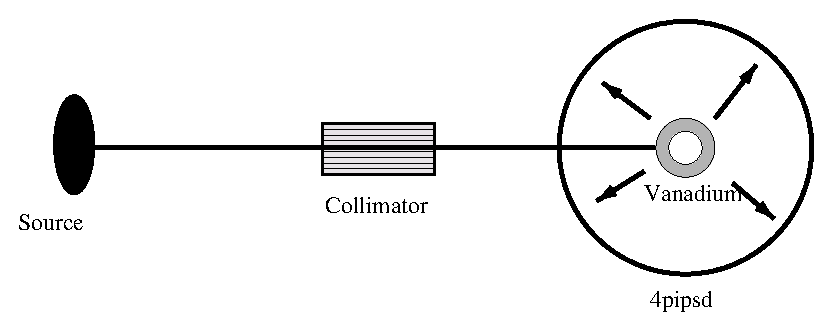
\includegraphics[width=0.9\textwidth]{figures/vanadium.eps}
  \end{center}
\caption{A sketch of the test instrument for the component
V\_sample.}
\label{f:V-instr}
\end{figure}

\subsection{Scattering from the V-sample test instrument}
\label{s:vanadium-result}

In figure \ref{f:V-results}, we present the radial distribution 
of the scatting from an evenly illuminated V-sample,
as seen by a spherical PSD.
It is interesting to note that the variation in the
scattering intensity is as large as 10\%. This is an effect
of attenuation of the beam in the cylindrical sample.

\begin{figure}
  \begin{center}
    \includegraphics[width=0.6\textwidth]{figures/vanadium-surf-2.eps}
  \end{center}
\caption{Scattering from a V-sample, measured by a spherical
  PSD. The sphere has been transformed onto a plane and the intensity is
  plotted as the third dimension. A colour version of this picture is
  found on the title page of this manual.}
\label{f:V-results}
\end{figure}



\section{The triple axis spectrometer TAS1}
\label{s:TAS1}
With this instrument definition, we have tried to create
a very detailed model of the conventional cold-source
triple-axis spectrometer TAS1 at Ris\o\ National Laboratory.
Unfortunately, no neutron scattering is performed at Ris\o\
anymore, but it still serves as a good example.
Except for the cold source itself, all components 
used have quite realistic properties. Furthermore, the overall
geometry of the instrument has been adapted from
the detailed technical drawings of the real spectrometer.
The TAS 1 simulation is the first detailed work
performed with the \MCS\ package.%, and a few of the simulation
%results are shown in Appendix \ref{testresults}.
For further details see reference~\cite{tas1_report}.

At the spectrometer, the channel from the cold source 
to the monochromator is asymmetric, since the first
part of the channel is shared with other instruments.
In the instrument definition, this is represented by
three slits.
For the cold source, we use a flat energy
distribution (component {\bf Source\_flat}) 
focusing on the third slit.

The real monochromator consist of seven blades, vertically focusing on
the sample. The angle of curvature is constant so that the focusing is
perfect at 5.0 meV (20.0 meV for 2nd order reflections) for a 1$\times$1~cm$^2$
sample. This is modeled directly in the instrument definition using
seven {\bf Monochromator} components. The mosaicity of the pyrolytic
graphite crystals is nominally 30' (FWHM) in both directions.  However, the
simulations indicated that the horisontal mosaicities of both
monochromator and analyser were more likely 45'. This was used for all
mosaicities in the final instrument definition.

The monochromator scattering angle, in effect determining the incoming
neutron energy, is for the real spectrometer fixed by four holes in the
shielding, corresponding to the energies 3.6, 5.0, 7.2, and 13.7~meV for
first order neutrons.  In the instrument definition, we have adapted the
angle corresponding to 5.0~meV in order to test the simulations against
measurements performed on the spectrometer.

The exit channel from the monochromator may 
on the spectrometer be narrowed down from initially 40~mm
to 20~mm by an insert piece. In the simulations, we have chosen
the 20~mm option and modeled the channel with two slits to match
the experimental set-up.

In the test experiments, we used two standard samples:
An Al$_2$O$_3$ powder sample and a vanadium sample. The instrument
definitions use either of these samples of the correct
size. Both samples are chosen to focus on the opening aperture of
collimator 2 (the one between the sample and the analyser).
Two slits, one before and one after the sample,
are in the instrument definition set to the opening values which
were used in the experiments.

The analyser of the spectrometer is flat and made from 
pyrolytic graphite. It is placed between an entry and 
an exit channel, the latter leading to a single detector.
All this has been copied into the instrument definition,
where the graphite mosaicity has been set to 45'.

On the spectrometer, Soller collimators may be inserted
at three positions: Between monochromator and sample,
between sample and analyser, and between analyser and detector.
In our instrument definition, we have used 30', 28', and 67' collimators
on these three positions, respectively.

An illustration of the TAS1 instrument
is shown in figure~\ref{f:TAS1}.
Test results and data from the real spectrometer are shown
in Appendix~\ref{data:TAS1}. 

\begin{figure}
  \begin{center}
    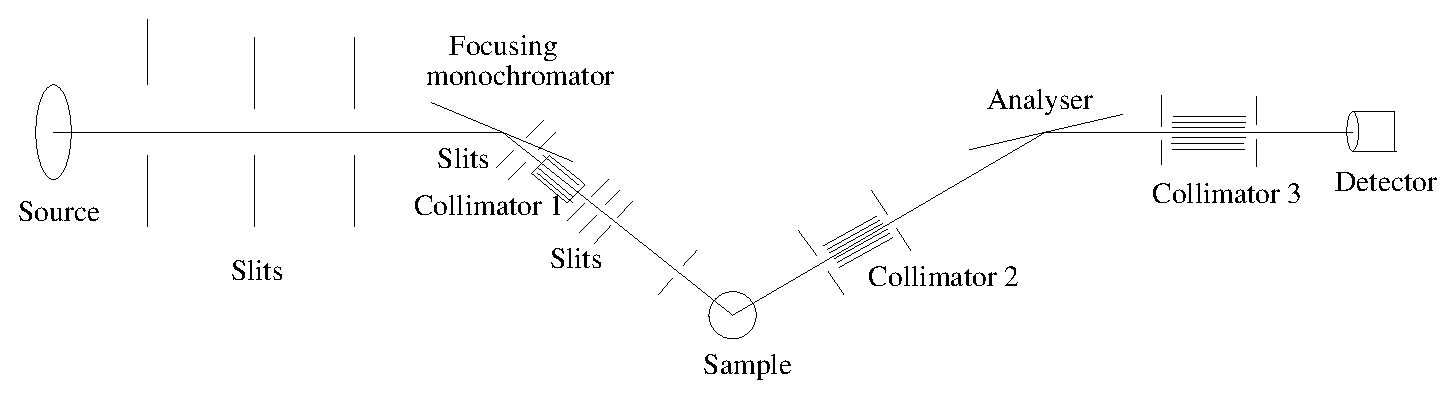
\includegraphics[width=0.9\textwidth]{figures/tas1.eps}
  \end{center}
\caption{A sketch of the TAS1 instrument.}
\label{f:TAS1}
\end{figure}

\subsection{Simulated and measured resolution of TAS1}
\label{data:TAS1}

In order to test the \MCS\ package on a qualitative level,
we have performed a very detailed simulation of the conventional
triple axis spectrometer TAS1, Ris\o . The measurement series
constitutes a complete alignment of the spectrometer,
using the direct beam and scattering from V and Al$_2$O$_3$
samples at an incoming energy of 20.0~meV, using the second order
scattering from the monochromator. 
In the instrument definitions, we have used all available
information about the spectrometer. However, the
mosaicities of the monochromator and analyser are set
to 45' in stead of the quoted 30', since we from our
analysis believe this to be much closer to the truth.

In these simulations, we have tried to reproduce
every alignment scan with respect to position and width
of the peaks, whereas we have not tried to compare
absolute intensities. Below, we show a few comparisons 
of the simulations and the measurements. 

Figure \ref{f:2t_direct} shows a scan of 
$2\theta_s$ on the collimated direct beam in two-axis mode.
A 1 mm slit is placed on the sample position.
Both the measured width and non-Gaussian peak shape
are well reproduced by the \MCS\ simulations.

\begin{figure}
  \begin{center}
    \includegraphics[width=0.6\textwidth]{figures/tas1-2T.eps}
  \end{center}
\caption{Scans of $2\theta_s$ in the direct beam with 1 mm slit on the
  sample position.
"$\times$": measurements, "o": simulations  
Collimations: open-30'-open-open.}
\label{f:2t_direct}
\end{figure}

In contrast, a simulated $2\theta_a$ scan in triple-axis 
mode on a V-sample showed a surprising offset from zero, see
Figure \ref{f:v_2ta_offset}. However, a simulation with a PSD
on the sample position showed that the beam center was 1.5~mm
off from the center of the sample, and this was important
since the beam was no wider than the sample itself.
A subsequent centering of the beam resulted in a nice
agreement between simulation and measurements. 
For a comparison on a slightly different instrument
(analyser-detector collimator inserted), 
see Figure~\ref{f:v_2ta_zero}.

\begin{figure}
  \begin{center}
    \includegraphics[width=0.6\textwidth]{figures/vanadium-plot-1.eps}
  \end{center}
\caption{First simulated $2\theta_a$ scan on a vanadium sample.
Collimations: open-30'-28'-open.}
\label{f:v_2ta_offset}
\end{figure}

\begin{figure}
  \begin{center}
    \includegraphics[width=0.6\textwidth]{figures/vanadium-plot-2.eps}
  \end{center}
\caption{Corrected $2\theta_a$ scan on a V-sample.
Collimations: open-30'-28'-67'.
"$\times$": measurements, "o": simulations.}
\label{f:v_2ta_zero}
\end{figure}

The result of a $2\theta_s$ scan on an Al$_2$O$_3$
powder sample in two-axis mode is shown in Figure \ref{f:al2o3}.
Both for the scan in focusing mode (+ $-$ +)
and for the one in defocusing mode (+ + +) (not shown),
the agreement between simulation and experiment is excellent.

\begin{figure}
  \begin{center}
    \includegraphics[width=0.6\textwidth]{figures/al2o3-focus.eps}
  \end{center}
\caption{$2\theta_s$ scans on Al$_2$O$_3$ in two-axis, focusing mode.
Collimations: open-30'-28'-67'.
"$\times$": measurements, "o": simulations.  
A constant background is added to the simulated data.}
\label{f:al2o3}
\end{figure}

As a final result, we present a scan of the energy
transfer $E_a = \hbar \omega$ on a V-sample.
The data are shown in Figure \ref{f:v_ea}.

\begin{figure}
  \begin{center}
    \includegraphics[width=0.6\textwidth]{figures/ea-scan.eps}
  \end{center}
\caption{Scans of the analyser energy on a V-sample.
Collimations: open-30'-28'-67'.
"$\times$": measurements, "o": simulations.}
\label{f:v_ea}
\end{figure}


\section{The time-of-flight spectrometer PRISMA}
\label{s:PRISMA} 

In order to test the time-of-flight aspect of \MCS, we have
in collaboration with Mark Hagen, ISIS, written a simple
simulation of a time-of-flight instrument loosely based on the ISIS
spectrometer PRISMA. The simulation was used to investigate the effect
of using a RITA-style analyser instead of the normal PRISMA backend.

We have used the simple time-of-flight source {\bf Tof\_source}. 
The neutrons pass through a
beam channel and scatter off from a vanadium sample, pass through
a collimator on to the analyser.
The RITA-style analyser consists of seven analyser crystals
that can be rotated independently around a vertical axis. After the
analysers we have placed a PSD and a time-of-flight detector.

To illustrate some of the things that can be done in a simulation as
opposed to a real-life experiment, this example instrument further
discriminates between
the scattering off each individual analyser crystal 
when the neutron hits the detector. The
analyser component is modified so that a global variable 
\verb+neu_color+ keeps track of which
crystal scatters the neutron. The detector component
is then modified to construct seven different time-of-flight histograms,
one for each crystal (see the source code for the instrument  
for details). One way to think of this is that
the analyser blades paint a color on each neutron which is then
observed in the detector.
An illustration of the instrument is shown in figure~\ref{f:PRISMA}.
Test results are shown in Appendix~\ref{data:PRISMA}.

\begin{figure}[h]
  \begin{center}
    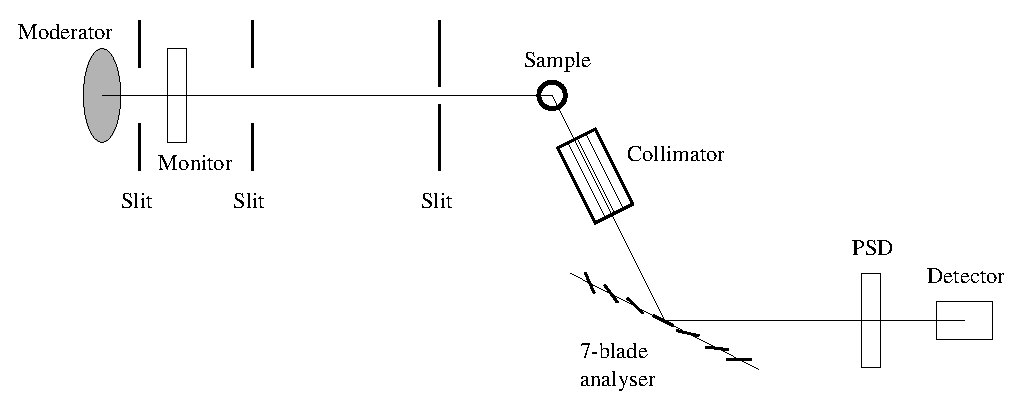
\includegraphics[width=0.9\textwidth]{figures/prisma2.eps}
  \end{center}
\caption{A sketch of the PRISMA instrument.}
\label{f:PRISMA}
\end{figure}

\subsection{Simple spectra from the PRISMA instrument}
\label{data:PRISMA}

A plot from the detector in the PRISMA simulation is shown in Figure
\ref{f:PRISMAdata}. These results were obtained with each analyser blade
rotated one degree relative to the previous one. The separation of the
spectra of the different analyser blades is caused by different energy
of scattered neutrons and different flight path length from source to
detector.  We have not performed any quantitative analysis of the data at this
time.

\begin{figure}
  \begin{center}
    \includegraphics[width=0.6\textwidth]{figures/prisma2-a.eps}
  \end{center}
\caption{Test result from PRISMA instrument using ``coloured
  neutrons''. Each graph shows the neutrons scattered from one analyser blade.}
\label{f:PRISMAdata}
\end{figure}

% Emacs settings: -*-mode: latex; TeX-master: "manual.tex"; -*-

\chapter{The component library:Abstract}
\label{s:components}
\index{Library!Components|textbf}

This chapter presents an abstract of existing components. As a complement to the \MCS\ component manual, you may use the \verb+mcdoc -s+ command to obtain the on-line component documentation and refer to the McStas web-page~\cite{mcstas_webpage} where all components are documented using the McDoc system.

\section{A short overview of the \MCS\ component library}
\label{s:comp-overview}

This section gives a quick overview of available \MCS\ components
provided with the distribution, in the \verb+MCSTAS+ library. The
location of this library is detailed in section~\ref{s:files}. All of them are thought to be reliable, eventhough no absolute guaranty may be given concerning their accuracy.\index{Environment variable!MCSTAS}

The \verb+contrib+ directory of the library contains components that were given by \MCS\ users, but are not validated yet. \index{Library!Components!contrib}

Additionally the \verb+obsolete+ directory of the library gathers components that were renamed, or considered to be outdated. Anyway, they still all work as before.
\index{Library!Components!obsolete}

The \verb+mcdoc+ front-end (section~\ref{s:mcdoc-run}) enables to display both the
catalog of the \MCS\ library, e.g using: \index{Tools!mcdoc}
\begin{quote}
  \verb|mcdoc|
\end{quote}
as well as the documentation of specific components, e.g with:
\begin{quote}
  \verb|mcdoc --text| {\it name} \\
  \verb|mcdoc| {\it file.comp}
\end{quote}
The first line will search for all components matching the {\it name}, and display their help section as text, where as the second example will display the help corresponding to the {\it file.comp} component, using your BROWSER\index{Environment variable!BROWSER} setting, or as text if unset. The \verb+--help+ option will display the command help, as usual.

\begin{table}
  \begin{center}
    {\let\my=\\
    \begin{tabular}{|p{0.24\textwidth}|p{0.7\textwidth}|}
      \hline
       {\bf MCSTAS/sources} & Description \\
       \hline
Adapt\_check & Optimization specifier for the Source\_adapt component. \\
ESS\_moderator\_long & Parametrised pulsed source for modelling ESS long pulses. \\
ESS\_moderator\_short & A parametrised pulsed source for modelling ESS short pulses. \\
Moderator  & A simple pulsed source for time-of-flight. \\
Monitor\_Optimizer &  To be used after the Source\_Optimizer component. \\
Source\_Maxwell\_3 & Source with up to three Maxwellian distributions \\
Source\_Optimizer & A component that optimizes the neutron flux passing through the Source\_Optimizer in order to have the maximum flux at the Monitor\_Optimizer position. \\
Source\_adapt  &       Neutron source with adaptive importance sampling. \\
Source\_div &          Neutron source with Gaussian divergence. \\
Source\_simple &  A simple circular neutron source with flat energy/wavelength spectrum.\\
Source\_gen     &    Circular/squared neutron source with flat or Maxwellian
                      energy/wavelength spectrum (possibly spatially
                      gaussian). \\
Virtual\_input &  Source-like component that generates neutron events from an ascii/binary 'virtual source' file (for Virtual\_output). \\
Virtual\_output &  Detector-like component that writes neutron state (for Virtual\_input). \\
      \hline
    \end{tabular}
    \caption{Source components of the \MCS\ library.}
    \label{t:comp-sources}
    \index{Library!Components!sources}
    }
  \end{center}
\end{table}


\begin{table}
  \begin{center}
    {\let\my=\\
    \begin{tabular}{|p{0.24\textwidth}|p{0.7\textwidth}|}
      \hline
       {\bf MCSTAS/optics} & Description \\
       \hline
Arm                &  Arm/optical bench \\
 Beamstop          &   Rectangular/circular
                      beam stop. \\
 Bender            &   Models a curved
                      neutron guide (shown straight). \\
 Chopper           &   Disk chopper. \\
 Collimator\_linear &  A simple analytical Soller collimator
                      (with triangular
                      transmission).  \\
 Collimator\_radial &  A radial Soller collimator.\\
 FermiChopper      &  Straight Fermi Chopper with
                        rotating frame. \\
 Filter\_gen        &   This components may
                      either set the flux
                      or change it (filter-like), using
                      an external data
                      file. \\
 Guide             &   Neutron guide. \\
 Guide\_channeled   &   Neutron guide with
                      channels (bender
                      section). \\
 Guide\_gravity     &  Neutron guide with gravity. Can be
                      channeled and focusing. \\

 Guide\_wavy        &   Neutron guide with
                      gaussian waviness. \\

 Mirror             &  Single mirror plate. \\


 Monochromator\_curved & Double bent multiple crystal
                      slabs with anisotropic gaussian
                      mosaic. \\

 Monochromator\_flat &  Flat Monochromator
                      crystal with
                      anisotropic mosaic. \\

 Selector            & A velocity selector
                      (helical lamella
                      type) such as
                      V\_selector component. \\

 Slit                & Rectangular/circular
                      slit. \\

 V\_selector          & Velocity selector. \\
 Vitess\_ChopperFermi & Curved Fermi chopper (slower than FermiChopper). From the Vitess package.\\
      \hline
    \end{tabular}
    \caption{Optics components of the \MCS\ library.}
    \label{t:comp-optics}
    \index{Library!Components!optics}
    }
  \end{center}
\end{table}

\begin{table}
  \begin{center}
    {\let\my=\\
    \begin{tabular}{|p{0.24\textwidth}|p{0.7\textwidth}|}
      \hline
       {\bf MCSTAS/samples} & Description \\
       \hline
  Isotropic\_Sqw & A general S(q,$\omega$) scatterer with multiple scattering, for liquids, powders, glasses, polymers. May be concentrically arranged. Coherent/incoherent, elastic/inelastic scattering. \\
  Phonon\_simple   & Acoustic phonon isotropic scatterer (simple). \\
  Powder1      &  General powder sample with a single
                scattering vector. \\
  Powder2      &  General powder sample with a two
                scattering vectors. \\
  PowderN      &  General powder sample with a N
                scattering vectors, using a data file. \\
  Res\_sample   & Sample for resolution function
                calculation. \\

  Sans\_spheres  & Sample for Small Angle Neutron Scattering - hard spheres in thin solution, mono disperse. \\

  Single\_crystal & Mosaic single crystal with multiple
                scattering vectors. \\
  TOFRes\_sample & Sample for resolution function
                calculation (TOF version). \\

  V\_sample      & Vanadium sample.\\
      \hline
    \end{tabular}
    \caption{Sample components of the \MCS\ library.}
    \label{t:comp-samples}
    \index{Library!Components!samples}
    }
  \end{center}
\end{table}

\begin{table}
  \begin{center}
    {\let\my=\\
    \begin{tabular}{|p{0.24\textwidth}|p{0.7\textwidth}|}
      \hline
       {\bf MCSTAS/monitors} & Description \\
       \hline
DivLambda\_monitor &  Divergence/wavelength monitor. \\
DivPos\_monitor  &    Divergence/position
                    monitor (acceptance
                    diagram). \\
Divergence\_monitor &  Horizontal+vertical
                    divergence monitor. \\
EPSD\_monitor    &    A monitor measuring neutron
                    intensity vs. position, x,
                    and neutron energy, E. \\
E\_monitor       &    Energy-sensitive monitor. \\
Hdiv\_monitor    &    Horizontal divergence monitor
L\_monitor           Wavelength-sensitive monitor. \\
Monitor          &   Simple
                    single detector/monitor. \\

Monitor\_4PI     &    Monitor that detects ALL
                    non-absorbed neutrons. \\
Monitor\_nD      &    This
                    component is a general
          Monitor that can output
                    0/1/2D signals (Intensity
                    or signal vs. [something]
                    and vs. [something] ...). \\
PSD\_monitor     &    Position-sensitive
                    monitor. \\
PSD\_monitor\_4PI  &   Spherical
                    position-sensitive
                    detector. \\
PSDcyl\_monitor  &    A 2D
                    Position-sensitive
                    monitor. The shape is
                    cylindrical with the axis
                    vertical. The monitor
                    covers the whole cylinder
                    (360 degrees). \\
PSDlin\_monitor   &   Rectangular 1D PSD,
                    measuring intensity vs.
                    vertical position, x. \\
PreMonitor\_nD    &   This component is a
                    PreMonitor that is to be
                    used with one Monitor\_nD,
                    in order to record some
                    neutron parameter correlations. \\
Res\_monitor      &   Monitor for resolution
                    calculations (Res\_sample and TOFRes\_sample). \\
TOFLambda\_monitor &  Time-of-flight/wavelength
                    monitor. \\
TOF\_cylPSD\_monitor & Cylindrical (2pi) PSD
                    Time-of-flight monitor. \\
TOF\_monitor     &    Rectangular Time-of-flight
                    monitor. \\
TOFlog\_mon      &    Rectangular Time-of-flight
                    monitor with logarithmic
                    time binning. \\
      \hline
    \end{tabular}
    \caption{Monitor components of the \MCS\ library.}
    \label{t:comp-monitors}
    \index{Library!Components!monitors}
    }
  \end{center}
\end{table}

\begin{table}
  \begin{center}
    {\let\my=\\
    \begin{tabular}{|p{0.24\textwidth}|p{0.7\textwidth}|}
      \hline
       {\bf MCSTAS/misc} & Description \\
       \hline
 Progress\_bar     &       A simulation
                      progress bar. May also trigger intermediate SAVE.\\
 Vitess\_input     &   Read neutron state
                      parameters from
                      VITESS neutron file.\\
 Vitess\_output    &  Write neutron state
     parameters to VITESS
                      neutron file.\\
      \hline
    \end{tabular}
    \caption{Miscellaneous components of the \MCS\ library.}
    \label{t:comp-misc}
    \index{Library!Components!misc}
    }
  \end{center}
\end{table}

\begin{table}
  \begin{center}
    {\let\my=\\
    \begin{tabular}{|p{0.24\textwidth}|p{0.7\textwidth}|}
      \hline
       {\bf MCSTAS/contrib} & Description \\
       \hline
 Al\_window     &         Aluminium
                        window in the beam. \\
 Collimator\_ROC   &      Radial
                        Oscillationg
                        Collimator (ROC). \\
 Filter\_graphite  &      Pyrolytic
                        graphite filter
                        (analytical model). \\
 Filter\_powder   &       Box-shaped powder
                        filter based on Single\_crystal (unstable). \\
 Guide\_curved     &     Non focusing continuous curved guide (shown curved). \\
 Guide\_honeycomb & Neutron guide
                        with gravity and
                        honeycomb geometry. Can be
                        channeled and
                        focusing. \\
 Guide\_tapering  &     Rectangular tapered guide (parabolic, elliptic, sections ...). \\

 He3\_cell    &           Polarised 3He cell. \\
 ISIS\_moderator    &     ISIS Target 1 and 2 moderator models based on MCNP calculations. \\
 Monochromator\_2foc   &  Double bent
                        monochromator with
                        multiple slabs. \\
 PSD\_monitor\_rad & A banana PSD monitor. \\
 SiC           &         SiC multilayer sample for reflectivity simulations. \\
 SNS\_source    & SNS moderator models based on MCNP calculations. \\
 Virtual\_tripoli4\_input & Reads a 'Batch' neutron events file from Tripoli 4. \\
 Virtual\_tripoli4\_output& Writes a 'Batch' neutron events file for Tripoli 4. \\

      \hline
    \end{tabular}
    \caption{Contributed components of the \MCS\ library.}
    \index{Library!Components!contrib}
    \label{t:comp-contrib}
    }
  \end{center}
\end{table}

\begin{table}
  \begin{center}
    {\let\my=\\
    \begin{tabular}{|p{0.24\textwidth}|p{0.7\textwidth}|}
      \hline
       {\bf MCSTAS/share} & Description \\
       \hline
       adapt\_tree-lib  & Handles a simulation optimisation space for
       adatative importance sampling.
                          Used by the Source\_adapt component. \\
       {\bf mcstas-r}      &   Main Run-time library (always included). \\
       monitor\_nd-lib & Handles multiple monitor types.
                        Used by Monitor\_nD, Res\_monitor, \ldots \\
       read\_table-lib  & Enables to read a data table (text/binary) to be used within
                          an instrument or a component. \\
       vitess-lib &     Enables to read/write Vitess event binary files.
                        Used by Vitess\_input and Vitess\_output \\
      \hline
    \end{tabular}
    \caption{Shared libraries of the \MCS\ library. See Appendix~\ref{c:kernelcalls} for details.}
    \label{t:comp-share}
    \index{Library!Components!share}
    \index{Library!Run-time}
    }
  \end{center}
\end{table}

\begin{table}
  \begin{center}
    {\let\my=\\
    \begin{tabular}{|p{0.24\textwidth}|p{0.7\textwidth}|}
      \hline
       {\bf MCSTAS/data} & Description \\
       \hline
 *.lau & Laue pattern file, as issued from Crystallographica or FullProf. Used e.g. for Powder1, PowderN, Single\_crystal
       Data: [ h   k   l Mult. d-space 2Theta   F-squared ] \\
 *.trm & transmission file, typically for monochromator crystals and filters.
       Data: [ k (Angs-1) , Transmission (0-1) ] \\
 *.rfl & reflectivity file, typically for mirrors and monochromator crystals.
       Data: [ k (Angs-1) , Reflectivity (0-1) ] \\
 *.sqw & Sample dynamical structure factors, e.g. for Isotropic\_Sqw. Data: Vector $q$, then vector $omega$, then matrix $S(q,\omega)$. \\
      \hline
    \end{tabular}
    \caption{Data files of the \MCS\ library.}
    \label{t:comp-data}
    \index{Library!Components!data}
    }
  \end{center}
\end{table}

\begin{table}
  \begin{center}
    {\let\my=\\
    \begin{tabular}{|p{0.24\textwidth}|p{0.7\textwidth}|}
      \hline
       {\bf MCSTAS/examples} & Description \\
      \hline
      *.instr & This directory contains example instruments, accessible throught the \verb+mcgui+ ``Neutron site'' menu. \\
      \hline
    \end{tabular}
    \caption{Instrument example files of the \MCS\ library.}
    \label{t:comp-instr}
    \index{Library!Instruments}
    }
  \end{center}
\end{table}

%\include{comp_future}

\appendix
% Emacs settings: -*-mode: latex; TeX-master: "manual.tex"; -*-

\chapter{Libraries and conversion constants}
\label{c:kernelcalls}
\index{Library|textbf}
\index{Library!Shared|see{Library/Components/share}}
\index{Library!mcstas-r|see{Library/Run-time}}

The \MCS\ Library contains a number of built-in functions
and conversion constants which are useful when constructing
components. These are stored in the \verb+share+ directory of
the \verb+MCSTAS+ library. \index{Library!Components!share}
\index{Environment variable!MCSTAS}

Within these functions, the 'Run-time' part is available for all
component/instrument descriptions. The other parts
% (see table~\ref{t:comp-share})
are dynamic, that is they are not
pre-loaded, but only imported once when a component requests it
using the \verb+%include+ \MCS\ keyword. For instance, within a
component C code block, (usually SHARE or DECLARE):
\index{Keyword!\%include}
\begin{verbatim}
    %include "read_table-lib"
\end{verbatim}
will include the 'read\_table-lib.h' file, and the 'read\_table-lib.c'
(unless the \verb+--no-runtime+ option is used with \verb+mcstas+).
Similarly,
\begin{verbatim}
    %include "read_table-lib.h"
\end{verbatim}
will \emph{only} include the 'read\_table-lib.h'.
The library embedding is done only once for all components (like the
 SHARE section). \index{Keyword!SHARE} For an example
of implementation, see {\bf Res\_monitor}.

In this Appendix, we present a short list of both each of the library contents
and the run-time features.

\section{Run-time calls and functions (\texttt{mcstas-r})}
\label{s:calls:run-time}
\index{Library!Run-time|textbf}
\index{Library!mcstas-r|see{Library/Run-time}}
Here we list a number of preprogrammed macros
which may ease the task of writing component and instrument definitions.

\subsection{Neutron propagation}
\index{Library!Run-time!SCATTER}
\index{Library!Run-time!ABSORB}
\index{Library!Run-time!PROP\_Z0}
\index{Library!Run-time!PROP\_DT}
\index{Library!Run-time!PROP\_GRAV\_DT}
\index{Library!Run-time!ALLOW\_BACKPROP}
Propagation routines perform all necessary operations to transport neutron rays
from one point to an other. Except when using the special
\verb+ALLOW_BACKPROP;+ call prior to exectuting any \verb+PROP_*+ propagation,
the neutron rays which have negative propagation times are removed automatically.
\begin{itemize}
\item {\bf ABSORB}. This macro issues an order to the overall
  \MCS\ simulator to interrupt the simulation of the current neutron
  history and to start a new one.
\item {\bf PROP\_Z0}. Propagates the neutron to the $z=0$ plane,
  by adjusting $(x,y,z)$ and $t$ accordingly from knowledge of the
  neutron velocity $(vx,vy,vz)$.
  If the propagation time is negative, the neutron ray is absorbed.

  For components that are centered along the $z$-axis,
  use the \verb+_intersect+ functions to determine intersection time(s),
  and then a \verb+PROP_DT+ call.
\item {\bf PROP\_DT}$(dt)$. Propagates the neutron through the
  time interval $dt$, adjusting $(x,y,z)$ and $t$ accordingly
  from knowledge of the neutron velocity.
\item {\bf PROP\_GRAV\_DT}$(dt,Ax,Ay,Az)$. Like {\bf PROP\_DT}, but it also
  includes gravity using the acceleration $(Ax,Ay,Az)$. In addition
  to adjusting $(x,y,z)$ and $t$, also $(vx,vy,vz)$ is modified.
\item {\bf ALLOW\_BACKPROP}. Indicates that the next propagation routine
  will not remove the neutron ray, even if negative propagation times
  are found. Further propagations are not affected.\index{Removed neutron events}
\item {\bf SCATTER}. This macro is used to denote a scattering event
  inside a component.
%, see section~\ref{s:comp-trace}.
  It should be used e.g
  to indicate that a component has interacted with the neutron ray
  (e.g. scattered or detected).
  This does not affect the simulation (see, however, {\bf Beamstop}),
  and it is mainly used by the
  \verb+MCDISPLAY+ section and the \verb+GROUP+ modifier
%(see~\ref{s:trace} and \ref{s:comp-mcdisplay}).
  See also the SCATTERED variable (below).
  \index{Keyword!GROUP} \index{Keyword!MCDISPLAY} \index{Keyword!EXTEND}
\end{itemize}

\subsection{Coordinate and component variable retrieval}
\index{Library!Run-time!MC\_GETPAR}
\index{Library!Run-time!NAME\_CURRENT\_COMP}
\index{Library!Run-time!POS\_A\_CURRENT\_COMP}
\index{Library!Run-time!ROT\_A\_CURRENT\_COMP}
\index{Library!Run-time!POS\_A\_COMP}
\index{Library!Run-time!ROT\_A\_COMP}
\index{Library!Run-time!STORE\_NEUTRON}
\index{Library!Run-time!RESTORE\_NEUTRON}
\index{Library!Run-time!SCATTERED}
\begin{itemize}
\item {\bf MC\_GETPAR}$(comp, outpar)$. This may be used in e.g. the FINALLY section of an
  instrument definition to reference the output parameters of a
  component.
% See page~\pageref{mcgetpar} for details.
\item {\bf NAME\_CURRENT\_COMP} gives the name of the current component as a string.
\item {\bf POS\_A\_CURRENT\_COMP} gives the absolute position of the
  current component. A component of the vector is referred to as
  POS\_A\_CURRENT\_COMP.$i$ where $i$ is $x$, $y$ or $z$.
\item {\bf ROT\_A\_CURRENT\_COMP} and
  {\bf ROT\_R\_CURRENT\_COMP} give the orientation
  of the current component as rotation matrices
  (absolute orientation and the orientation relative to
  the previous component, respectively). A
  component of a rotation matrix is referred to as
  ROT\_A\_CURRENT\_COMP$[m][n]$, where $m$ and
  $n$ are 0, 1, or 2 standing for $x,y$ and $z$ coordinates respectively.
\item {\bf POS\_A\_COMP}$(comp)$ gives the absolute position
  of the component with the name {\em comp}. Note that
  {\em comp} is not given as a string. A component of the
  vector is referred to as POS\_A\_COMP$(comp).i$
  where $i$ is $x$, $y$ or $z$.
\item {\bf ROT\_A\_COMP}$(comp)$ and
  {\bf ROT\_R\_COMP}$(comp)$ give the orientation of the
  component {\em comp} as rotation matrices (absolute
  orientation and the orientation relative to its
  previous component, respectively). Note that {\em comp}
  is not given as a string. A component of  a rotation
  matrice is referred to as
  ROT\_A\_COMP$(comp)[m][n]$, where $m$ and $n$ are
  0, 1, or 2.
\item {\bf INDEX\_CURRENT\_COMP} is the number (index) of the
       current component  (starting from 1).
\item {\bf POS\_A\_COMP\_INDEX}$(index)$ is the absolute position of
  component $index$. \\
  POS\_A\_COMP\_INDEX (INDEX\_CURRENT\_COMP) is the same as \\
  POS\_A\_CURRENT\_COMP. You may use \\
  POS\_A\_COMP\_INDEX  (INDEX\_CURRENT\_COMP+1) \\
  to make, for instance, your
  component access the position of the next component (this is usefull for
  automatic targeting).  A component of the vector is referred to as
  POS\_A\_COMP\_INDEX$(index).i$ where $i$ is $x$, $y$ or $z$.
\item {\bf POS\_R\_COMP\_INDEX} works the same as above,
  but with relative coordinates.
\item {\bf STORE\_NEUTRON}$(index, x, y, z, vx, vy, vz, t$, $sx, sy,
sz, p)$ stores the current neutron state in the trace-history table,
in local coordinate system. $index$ is usually INDEX\_CURRENT\_COMP.
This is automatically done when entering each component of an
instrument.
\item {\bf RESTORE\_NEUTRON}$(index, x, y, z, vx, vy, vz, t, sx, sy,
sz, p)$ restores the neutron state to the one at the input of the
component $index$. To ignore a component effect, use
RESTORE\_NEUTRON (INDEX\_CURRENT\_COMP, \\
$x, y, z, vx, vy, vz, t,
sx, sy, sz, p$) at the end of its TRACE section, or in its EXTEND
section. These neutron states are in the local component coordinate
systems.
\item {\bf SCATTERED} is a variable set to 0 when entering
  a component, which is incremented each time a SCATTER event occurs.
  This may be used in the \verb+EXTEND+ sections to determine whether
  the component interacted with the current neutron ray.
\item {\bf extend\_list}($n$, \&\textit{arr}, \&\textit{len},
  \textit{elemsize}). Given an array \textit{arr} with \textit{len}
  elements each of size \textit{elemsize}, make sure that the array is
  big enough to hold at least $n$ elements, by extending \textit{arr}
  and \textit{len} if necessary. Typically used when reading a list of
  numbers from a data file when the length of the file is not known in advance.
\item {\bf mcset\_ncount}$(n)$. Sets the number of neutron histories to simulate to $n$.
\item {\bf mcget\_ncount}(). Returns the number of neutron histories to simulate (usually set by option \verb+-n+).
\item {\bf mcget\_run\_num}(). Returns the number of neutron histories that have been simulated until now.
\end{itemize}

\subsection{Coordinate transformations}
\begin{itemize}
\item {\bf coords\_set}$(x,y,z)$ returns a Coord structure (like POS\_A\_CURRENT\_COMP) with $x$, $y$ and $z$ members.
\item {\bf  coords\_get}$(P,$ \&$x$, \&$y$, \&$z)$ copies the $x$, $y$ and
$z$ members of the Coord structure $P$ into $x,y,z$ variables.
\item {\bf coords\_add}$(a,b)$, {\bf coords\_sub}$(a,b)$, {\bf
coords\_neg}$(a)$ enable to  operate on coordinates, and return the
resulting Coord structure.
\item {\bf rot\_set\_rotation}({\it Rotation t}, $\phi_x, \phi_y, \phi_z$)
  Get transformation matrix for rotation
  first $\phi_x$ around x axis, then $\phi_y$ around y,
  and last $\phi_z$ around z. $t$ should be a 'Rotation' ([3][3] 'double' matrix).
\item {\bf rot\_mul}{\it (Rotation t1, Rotation t2, Rotation t3)} performs $t3 = t1 . t2$.
\item {\bf rot\_copy}{\it (Rotation dest, Rotation src)} performs $dest = src$ for Rotation arrays.
\item {\bf rot\_transpose}{\it (Rotation src, Rotation dest)} performs $dest = src^t$.
\item {\bf rot\_apply}{\it (Rotation t, Coords a)} returns a Coord structure which is $t.a$
\end{itemize}

\subsection{Mathematical routines}
\begin{itemize}
\item {\bf NORM}$(x,y,z)$. Normalizes the vector $(x,y,z)$ to have
  length 1.
\item {\bf scalar\_prod}$(a_x,a_y,a_z,b_x,b_y,b_z)$. Returns the scalar
  product of the two vectors $(a_x,a_y,a_z)$ and $(b_x,b_y,b_z)$.
\item {\bf vec\_prod}$(a_x,a_y,a_z,b_x,b_y,b_z, c_x,c_y,c_z)$. Sets
  $(a_x,a_y,a_z)$ equal to the vector product $(b_x,b_y,b_z) \times (c_x,c_y,c_z)$.
\item {\bf rotate}$(x,y,z,v_x,v_y,v_z,\varphi,a_x,a_y,a_z)$. Set
  $(x,y,z)$ to the result of rotating the vector $(v_x,v_y,v_z)$
  the angle $\varphi$ (in radians) around the vector $(a_x,a_y,a_z)$.
\item {\bf normal\_vec}(\&$n_x$, \&$n_y$, \&$n_z$, $x$, $y$, $z$).
  Computes a unit vector $(n_x, n_y, n_z)$ normal to the vector
  $(x,y,z)$.
\item {\bf solve\_2nd\_order}(*$t$, $A$,  $B$,  $C$).
  Solves the 2$^{nd}$ order equation $At^2 + Bt + C = 0$ and returns
  the smallest positive solution into pointer *$t$.
\end{itemize}

\subsection{Output from detectors}
Details about using these functions are given in the \MCS\ User Manual.
\begin{itemize}
\item {\bf DETECTOR\_OUT\_0D}$(...)$. Used to output the results from a
  single detector. The name of the detector is output together
  with the simulated intensity and estimated statistical error. The
  output is produced in a format that can be read by \MCS\ front-end
  programs.
%See section~\ref{s:comp-finally} ??? for details.
\item {\bf DETECTOR\_OUT\_1D}$(...)$. Used to output the results from a
  one-dimentional detector.
%See section~\ref{s:comp-finally} for details.
\item {\bf DETECTOR\_OUT\_2D}$(...)$. Used to output the results from a
  two-dimentional detector.
%See section~\ref{s:comp-finally} for details.
\item {\bf DETECTOR\_OUT\_3D}$(...)$. Used to output
  the results from a three-dimentional detector. Arguments are the same as
  in DETECTOR\_OUT\_2D, but with the additional $z$ axis (the signal).
  Resulting data files are treated as 2D data, but the 3rd dimension is
  specified in the $type$ field.
\item {\bf mcinfo\_simulation}{\it (FILE *f, mcformat,
  char *pre, char *name)} is used to append the simulation parameters into file $f$
  (see for instance {\bf Res\_monitor}).
  Internal variable $mcformat$ should be used as specified.
  Please contact the authors for further information.
\end{itemize}

\subsection{Ray-geometry intersections}
\begin{itemize}
\item {\bf inside\_rectangle}(\&$x$, \&$y$, $x$, $xw$, $yh$). 
  Return 1 if $-xw/2 \leq x \leq xw/2$ AND $-yh/2 \leq y \leq yh/2$. 
  Else return 0.
\item {\bf box\_intersect}(\&$t_1$, \&$t_2$, $x$, $y$, $z$, $v_x$, $v_y$, $v_z$,
  $d_x$, $d_y$, $d_z$). Calculates the (0, 1, or 2) intersections between
  the neutron path and a box of dimensions $d_x$, $d_y$, and $d_z$,
  centered at the origin for a neutron with the parameters
  $(x,y,z,v_x,v_y,v_z)$. The times of intersection are returned
  in the variables $t_1$ and $t_2$, with $t_1 < t_2$. In the case
  of less than two intersections, $t_1$ (and possibly $t_2$) are set to
  zero. The function returns true if the neutron intersects the box,
  false otherwise.
\item {\bf cylinder\_intersect}(\&$t_1$, \&$t_2$, $x$, $y$, $z$, $v_x$, $v_y$, $v_z$,
  $r$, $h$).  Similar to {\bf box\_intersect}, but using a cylinder of height $h$ and radius $r$,
  centered at the origin.
\item {\bf sphere\_intersect}(\&$t_1$, \&$t_2$, $x$, $y$, $z$, $v_x$, $v_y$, $v_z$,
  $r$). Similar to {\bf box\_intersect}, but using a sphere
  of radius $r$.
\end{itemize}

\subsection{Random numbers}
\begin{itemize}
\item {\bf rand01}(). Returns a random number distributed uniformly between 0 and 1.
\item {\bf randnorm}(). Returns a random number from a normal
  distribution centered around 0 and with $\sigma=1$. The algorithm used to
  get the normal distribution is explained in Ref.~\cite[ch.7]{num_rep}.
\item {\bf randpm1}(). Returns a random number distributed uniformly between -1 and 1.
\item {\bf randvec\_target\_circle}(\&$v_x$, \&$v_y$, \&$v_z$, \&$d\Omega$,
  aim$_x$, aim$_y$, aim$_z$, $r_f$). Generates a random vector $(v_x, v_y,
  v_z)$, of the same length as (aim$_x$, aim$_y$, aim$_z$), which is
  targeted at a \emph{disk} centered at (aim$_x$, aim$_y$, aim$_z$) with
  radius $r_f$ (in meters), and perpendicular to the \emph{aim} vector.. All directions
  that intersect the circle are chosen with equal probability. The solid
  angle of the circle as seen from the position of the neutron is returned
  in $d\Omega$. This routine was previously called {\bf randvec\_target\_sphere}
  (which still works).
\item {\bf randvec\_target\_rect\_angular}(\&$v_x$, \&$v_y$, \&$v_z$,
  \&$d\Omega$, aim$_x$, aim$_y$, aim$_z$,$h, w, Rot$) does the same as
  randvec\_target\_circle but targetting at a rectangle with angular dimensions
  $h$ and $w$ (in {\bf radians}, not in degrees as other angles). The
  rotation matrix $Rot$ is the coordinate system orientation in the absolute
  frame, usually ROT\_A\_CURRENT\_COMP.
\item {\bf randvec\_target\_rect}(\&$v_x$, \&$v_y$, \&$v_z$,
  \&$d\Omega$, aim$_x$, aim$_y$, aim$_z$,$height, width, Rot$) is the same as
  randvec\_target\_rect\_angular but $height$ and $width$ dimensions are given
  in meters. This function is useful to e.g. target at a guide entry window
  or analyzer blade.
\end{itemize}

\section{Reading a data file into a vector/matrix (Table input, \texttt{read\_table-lib})}
\label{s:read-table}
\index{Library!read\_table-lib (Read\_Table)|textbf}
  The \verb+read_table-lib+ provides functionalities for reading text
  (and binary) data files. To use this library,
  add a \verb+%include "read_table-lib"+ in your component definition
  DECLARE or SHARE section. Tables are structures of type $t_{\rm Table}$
  (see \verb+read_table-lib.h+ file for details):
\begin{verbatim}
    /* t_Table structure (most important members) */
    double *data;     /* Use Table_Index(Table, i j) to extract [i,j] element */
    long    rows;     /* number of rows */
    long    columns;  /* number of columns */
    char   *header;   /* the header with comments */
    char   *filename; /* file name or title */
    double  min_x;    /* minimum value of 1st column/vector */
    double  max_x;    /* maximum value of 1st column/vector */
\end{verbatim}

Available functions to read \emph{a single} vector/matrix are:
\begin{itemize}
\item {\bf Table\_Init}(\&$Table$, $rows$, $columns$) returns an allocated
  Table structure. Use $rows=columns=0$ not to allocate memory and return an empty table.
  Calls to Table\_Init are \emph{optional}, since initialization is being
  performed by other functions already.
\item {\bf Table\_Read}(\&$Table$, $filename$, $block$)
  reads numerical block number
  $block$ (0 to catenate all) data from \emph{text} file $filename$ into $Table$,
  which is as well initialized in the process.
  The block number changes when the numerical data changes its size,
  or a comment is encoutered (lines starting
  by '\verb+# ; % /+'). If the data could not be read,
  then $Table.data$ is NULL and $Table.rows = 0$.
  You may then try to read it using Table\_Read\_Offset\_Binary.
  Return value is the number of elements read.
\item {\bf Table\_Read\_Offset}(\&$Table$, $filename$, $block$, \&\textit{offset}, $n_{rows}$)
  does the same as Table\_Read except that it starts at offset \textit{offset}
  (0 means begining of file) and reads $n_{rows}$ lines (0 for all).
  The \textit{offset} is returned as the final offset reached after
  reading the $n_{rows}$ lines.
\item {\bf Table\_Read\_Offset\_Binary}(\&$Table$, $filename$, $type$,
  $block$, \&\textit{offset}, $n_{rows}$, $n_{columns}$) does the same as
  Table\_Read\_Offset, but also specifies the $type$ of the file (may
  be "float" or "double"), the number $n_{rows}$ of rows to read, each
  of them having $n_{columns}$ elements. No text header should be present
  in the file.
\item {\bf Table\_Rebin}(\&$Table$) rebins all $Table$ rows with increasing, evenly spaced first column (index 0), e.g. before using Table\_Value. Linear interpolation is performed for all other columns. The number of bins for the rebinned table is determined from the smallest first column step.
\item {\bf Table\_Info}$(Table)$ print information about the table $Table$.
\item {\bf Table\_Index}($Table, m, n$) reads the $Table[m][n]$ element.
\item {\bf Table\_Value}($Table, x, n$) looks for the closest $x$
  value in the first column (index 0), and extracts in this row the
  $n$-th element (starting from 0). The first column is thus the 'x' axis for the data. It does not contain any interpolation method.
\item {\bf Table\_Free}(\&$Table$) free allocated memory blocks.
\end{itemize}

Available functions to read \emph{an array} of vectors/matrices in a \emph{text} file are:
\begin{itemize}
\item {\bf Table\_Read\_Array}($File$, \&$n$) read and split $file$
into as many blocks as necessary and return a $t_{\rm Table}$ array.
Each block contains a single vector/matrix. This only works for text files.
The number of blocks in put into $n$.
\item {\bf Table\_Free\_Array}(\&$Table$) free the $Table$ array.
\item {\bf Table\_Info\_Array}(\&$Table$) display information about all data blocks.
\end{itemize}

The format of text files is free. Lines starting by '\verb+# ; % /+' characters are considered to be comments, and stored in $Table.header$. Data blocks are vectors and matrices. Block numbers are counted starting from 1, and changing when a comment is found, or the column number changes. For instance, the file 'MCSTAS/data/BeO.trm' (Transmission of a Berylium filter) looks like:
\begin{verbatim}
  # BeO transmission, as measured on IN12
  # Thickness: 0.05 [m]
  # [ k(Angs-1) Transmission (0-1) ]
  # wavevector multiply
  1.0500  0.74441
  1.0750  0.76727
  1.1000  0.80680
  ...
\end{verbatim}
Binary files should be of type "float" (i.e. REAL*32) and "double" (i.e. REAL*64),
and should \emph{not} contain text header lines. These files are platform
dependent (little or big endian).

The $filename$ is first searched into the current directory (and all user additional locations specified using the \verb+-I+ option, see the 'Running \MCS\ ' chapter in the User Manual), and if not found, in the \verb+data+ sub-directory of the \verb+MCSTAS+ library location. \index{Library!Components!data}
\index{Environment variable!MCSTAS} This way, you do not need to have local copies of the \MCS\ Library Data files (see table~\ref{t:comp-data}).

A usage example for this library part may be:
\begin{verbatim}
  t_Table Table;       // declare a t_Table structure
  char file[]="BeO.trm";  // a file name
  double x,y;

  Table_Read(&Table, file, 1);  // initialize and read the first numerical block
  Table_Info(Table);            // display table informations
  ...
  x = Table_Index(Table, 2,5);  // read the 3rd row, 6th column element
                                // of the table. Indexes start at zero in C.
  y = Table_Value(Table, 1.45,1);  // look for value 1.45 in 1st column (x axis)
                                // and extract 2nd column value of that row
  Table_Free(&Table);           // free allocated memory for table
\end{verbatim}
Additionally, if the block number (3rd) argument of  {\bf Table\_Read} is 0, all blocks will be catenated.
The {\bf Table\_Value} function assumes that the 'x' axis is the first column (index 0).
Other functions are used the same way with a few additional parameters, e.g. specifying an offset for reading files, or reading binary data.

This other example for text files shows how to read many data blocks:
\begin{verbatim}
  t_Table *Table;       // declare a t_Table structure array
  long     n;
  double y;

  Table = Table_Read_Array("file.dat", &n); // initialize and read the all numerical block
  n = Table_Info_Array(Table);     // display informations for all blocks (also returns n)

  y = Table_Index(Table[0], 2,5);  // read in 1st block the 3rd row, 6th column element
                                   // ONLY use Table[i] with i < n !
  Table_Free_Array(Table);         // free allocated memory for Table
\end{verbatim}

You may look into, for instance, the source files for
{\bf Monochromator\_curved} or {\bf Virtual\_input}
for other implementation examples.

\section{Monitor\_nD Library}
\index{Library!monitor\_nd-lib}

This library gathers a few functions used by a set of monitors e.g. Monitor\_nD, Res\_monitor, Virtual\_output, etc.
It may monitor any kind of data, create the data files, and may display many geometries (for \verb+mcdisplay+).
Refer to these components for implementation examples, and ask the authors for more details.

\section{Adaptative importance sampling Library}
\index{Library!adapt\_tree-lib}

This library is currently only used by the components {\bf Source\_adapt}
and {\bf Adapt\_check}. It performs adaptative importance sampling of neutrons for simulation efficiency optimization.
Refer to these components for implementation examples, and ask the authors for more details.

\section{Vitess import/export Library}
\index{Library!vitess-lib}

This library is used by the components
{\bf Vitess\_input} and {\bf Vitess\_output},
as well as the \verb+mcstas2vitess+ utility.
% (see section~\ref{s:mcstas2vitess}).
\index{Tools!mcstas2vitess}
Refer to these components for implementation examples, and ask the authors for more details.

\section{Constants for unit conversion etc.}
The following predefined constants are useful for conversion
between units
\def\textvb{\textbf}
\begin{center}
\begin{tabular}{|l|c|p{0.29\textwidth}|p{0.252\textwidth}|}
\hline
Name & Value & Conversion from & Conversion to \\ \hline
\textvb{DEG2RAD} & $2 \pi / 360$ & Degrees & Radians \\
\textvb{RAD2DEG} & $360 / (2 \pi)$ & Radians & Degrees \\
\textvb{MIN2RAD} & $2 \pi / (360 \cdot 60)$
  & Minutes of arc & Radians \\
\textvb{RAD2MIN} & $(360\cdot 60) / (2 \pi)$
  & Radians & Minutes of arc \\
\textvb{V2K} & $10^{10} \cdot m_{\rm N}/\hbar$
  & Velocity (m/s) & {\bf k}-vector (\AA$^{-1}$) \\
\textvb{K2V} & $10^{-10} \cdot \hbar / m_{\rm N}$
  & {\bf k}-vector (\AA$^{-1}$) & Velocity (m/s) \\
\textvb{VS2E} & $m_{\rm N} / (2 e)$
  & Velocity squared (m$^2$ s$^{-2}$) & Neutron energy (meV) \\
\textvb{SE2V} & $\sqrt{2 e/m_{\rm N}}$
  & Square root of neutron energy (meV$^{1/2}$) & Velocity (m/s) \\
\textvb{FWHM2RMS} & $1/\sqrt{8\log(2)}$
  & Full width half maximum & Root mean square (standard deviation) \\
\textvb{RMS2FWHM} & $\sqrt{8\log(2)}$
  & Root mean square (standard deviation) & Full width half maximum \\
\textvb{MNEUTRON} & $1.67492 \cdot 10^{-27}$~kg
  & Neutron mass, $m_{\rm n}$ & \\
\textvb{HBAR} & $1.05459 \cdot 10^{-34}$~Js
  & Planck constant, $\hbar$ & \\
\textvb{PI} & $3.14159265...$
  & $\pi$ & \\
\textvb{FLT\_MAX} & 3.40282347E+38F
  & a big float value & \\
\hline
\end{tabular}
\end{center}
 % as in manual
%% Emacs settings: -*-mode: latex; TeX-master: "manual.tex"; -*-

\chapter{\MCS\ source code for the component library}
\label{compcode}

\section*{List of component input and output parameters}

Before listing the source code for the components, we
bring a list of the components with their input and output parameters.

\begin{center}
\begin{tabular}{|ll|}
\hline
Source\_flat & \textbf{Input:} (radius, dist, xw, yh, E0, dE) \\
 & \textbf{Output:} (hdiv, vdiv, p\_in) \\
\hline
Source\_flat\_lambda & \textbf{Input:} (radius, dist, xw, yh, lambda\_0, d\_lambda) \\
 & \textbf{Output:} (hdiv, vdiv, p\_in) \\
\hline
Source\_flux\_lambda & \textbf{Input:} (radius, dist, xw, yh, lambda\_0,
    d\_lambda, flux) \\
 & \textbf{Output:} (hdiv, vdiv, p\_in) \\
\hline
Source\_div & \textbf{Input:} (width, height, hdiv, vdiv, E0, dE) \\
\hline
Moderator & \textbf{Input:} (radius, E0, E1, dist, xw, yh, t0, Ec, gam) \\
\hline
Source\_adapt & \textbf{Input:} (xmin, xmax, ymin, ymax, dist, xw, yh, E0, dE, flux) \\
     & \phantom{\textbf{Input:}\ }(n\_E, N\_xpos, N\_xdiv, alpha, beta, filename) \\
\hline
Arm & \textbf{Input:} () \\
\hline
Slit & \textbf{Input:} (xmin, xmax, ymin, ymax) \\
\hline
Circular\_slit & \textbf{Input:} (radius) \\
\hline
Beamstop\_rectangular & \textbf{Input:} (xmin, xmax, ymin, ymax) \\
\hline
Beamstop\_circular & \textbf{Input:} (radius) \\
\hline
Soller & \textbf{Input:} (xmin, xmax, ymin, ymax, len, divergence) \\
\hline
Filter & \textbf{Input:} (xmin, xmax, ymin, ymax, len, T0, T1, Emin, Emax) \\
\hline
Mirror & \textbf{Input:} (xlength, yheight, R0, Qc, alpha, m, W) \\
\hline
Guide & \textbf{Input:} (w1, h1, w2, h2, l, R0, Qc, alpha, m, W) \\
\hline
Channeled\_Guide & \textbf{Input:} (w1, h1, w2, h2, l, d, k) \\
                 & \phantom{\textbf{Input:}\ }(R0, Qcx, Qcy, alphax, alphay, mx, my, W) \\
\hline
\end{tabular}
\end{center}
\vfill
\begin{center}
\begin{tabular}{|ll|}
\hline
V\_selector & \textbf{Input:} (width, height, l0, r0, phi, l1, tb, rot, nb) \\
\hline
Chopper & \textbf{Input:} (w, R, f, n, pha) \\
 & \textbf{Output:} (Tg, To) \\
\hline
First\_Chopper & \textbf{Input:} (w, R, f, n, pha, a) \\
 & \textbf{Output:} (Tg, To) \\
\hline
Monitor & \textbf{Input:} (xmin, xmax, ymin, ymax) \\
 & \textbf{Output:} (Nsum, psum, p2sum) \\
\hline
Monitor\_4PI & \textbf{Output:} (Nsum, psum, p2sum) \\
\hline
PSD\_monitor & \textbf{Input:} (xmin, xmax, ymin, ymax, nx, ny, filename) \\
 & \textbf{Output:} (PSD\_N, PSD\_p, PSD\_p2) \\
\hline
PSD\_monitor\_4PI & \textbf{Input:} (radius, nx, ny, filename) \\
 & \textbf{Output:} (PSD\_N, PSD\_p, PSD\_p2) \\
\hline
PSD\_monitor\_4PI\_log & \textbf{Input:} (radius, nx, ny, filename) \\
 & \textbf{Output:} (PSD\_N, PSD\_p, PSD\_p2) \\
\hline
TOF\_monitor & \textbf{Input:} (xmin, xmax, ymin, ymax, nchan, dt, filename) \\
 & \textbf{Output:} (TOF\_N, TOF\_p, TOF\_p2) \\
\hline
E\_monitor & \textbf{Input:} (xmin, xmax, ymin, ymax, Emin, Emax, nchan, filename) \\
 & \textbf{Output:} (E\_N, E\_p, E\_p2) \\
\hline
L\_monitor & \textbf{Input:} (xmin, xmax, ymin, ymax, Lmin, Lmax, nchan, filename) \\
 & \textbf{Output:} (L\_N, L\_p, L\_p2) \\
\hline
Divergence\_monitor & \textbf{Input:} (xmin, xmax, ymin, ymax, nh, nv) \\
           & \phantom{\textbf{Input:}\ }(h\_maxdiv, v\_maxdiv, filename) \\
 & \textbf{Output:} (Div\_N, Div\_p, Div\_p2) \\
\hline
DivPos\_monitor & \textbf{Input:} (xmin, xmax, ymin, ymax, 
                       npos, ndiv, maxdiv, filename) \\
 & \textbf{Output:} (Div\_N, Div\_p, Div\_p2) \\
\hline
DivLambda\_monitor & \textbf{Input:} (xmin, xmax, ymin, ymax, nlam, ndiv, maxdiv) \\
          & \phantom{\textbf{Input:}\ }(lambda\_0, lambda\_1, filename) \\
 & \textbf{Output:} (Div\_N, Div\_p, Div\_p2) \\
\hline
Res\_monitor & \textbf{Input:} (xmin, xmax, ymin, ymax, filename, res\_sample\_comp) \\
 & \textbf{Output:} (Nsum, psum, p2sum, file) \\
\hline
Adapt\_check & \textbf{Input:} (source\_comp) \\
\hline
Mosaic\_simple & \textbf{Input:} (zmin, zmax, ymin, ymax, mosaic, R0, Qx, Qy, Qz) \\
\hline
Mosaic\_anisotropic & \textbf{Input:} (zmin, zmax, ymin, ymax, mosaich, mosaicv, r0, Q) \\
\hline
Single\_crystal & \textbf{Input:} (xwidth, yheight, zthick, delta\_d\_d, mosaic) \\
 & \phantom{\textbf{Input:}\ }(ax, ay, az, bx, by, bz, cx, cy, cz, reflections) \\
\hline
V\_sample & \textbf{Input:} (radius\_i,radius\_o,h,pack,focus\_r) \\
 & \phantom{\textbf{Input:}\ }(target\_x, target\_y, target\_z) \\
\hline
Powder1 & \textbf{Input:} (d\_phi0, radius, h, pack, Vc, sigma\_a, j, q, F2, DW) \\
 & \phantom{\textbf{Input:}\ }(target\_x, target\_y, target\_z) \\
 & \textbf{Output:} (my\_s\_v2, my\_a\_v, q\_v) \\
\hline
Res\_sample & \textbf{Input:} (radius\_i, radius\_o, h, focus\_r, E0, dE) \\
 & \phantom{\textbf{Input:}\ }(target\_x, target\_y, target\_z) \\
 & \textbf{Output:} (res\_struct) \\
\hline
\end{tabular}
\end{center}

\newpage

\section{Source components}

\subsection{Source\_flat}
\smallverbatimfile{../components/Source_flat.comp}
\newpage

\addtocounter{subsection}{1}    % Skip Source_flat_lambda

\subsection{Source\_flux\_lambda}
\smallverbatimfile{../components/Source_flux_lambda.comp}
\newpage

\subsection{Source\_div}
\smallverbatimfile{../components/Source_div.comp}
\newpage

\subsection{Moderator}
\smallverbatimfile{../components/Moderator.comp}
\newpage

\subsection{Source\_adapt}
\smallverbatimfile{../components/Source_adapt.comp}
\newpage

\addtocounter{subsection}{1}    % Skip Source_optimizer

\section{Simple components}

\subsection{Arm}
\label{code:arm}
\smallverbatimfile{../components/Arm.comp}
\newpage

\subsection{Slit}
\smallverbatimfile{../components/Slit.comp}
\newpage

\addtocounter{subsection}{1}    % Skip Circular_slit
%\subsection{Circular\_slit}
%\smallverbatimfile{../components/Circular_slit.comp}
%\newpage

\addtocounter{subsection}{1}    % Skip Beamstop_rectangular
\addtocounter{subsection}{1}    % Skip Beamstop_circular

\subsection{Soller}
\smallverbatimfile{../components/Soller.comp}
\newpage

\subsection{Filter}
\smallverbatimfile{../components/Filter.comp}
\newpage

\section{Beam optical components}
\addtocounter{subsection}{1}    % Skip mirror reflectivity

\addtocounter{subsection}{1}    % Skip Mirror
%\subsection{Mirror}
%\smallverbatimfile{../components/Mirror.comp}
%\newpage

\subsection{Guide}
\smallverbatimfile{../components/Guide.comp}
\newpage

\subsection{Channeled\_Guide}
\smallverbatimfile{../components/Channeled_guide.comp}
\newpage

\section{Chopper-like components}
\subsection{V\_selector.comp}
\smallverbatimfile{../components/V_selector.comp}
\newpage

\subsection{Chopper.comp}
\smallverbatimfile{../components/Chopper.comp}
\newpage

\addtocounter{subsection}{1}    % Skip First_Chopper
%\subsection{First\_Chopper.comp}
%\smallverbatimfile{../components/First_Chopper.comp}
%\newpage

\section{Detectors and monitors}
\subsection{Monitor}
\smallverbatimfile{../components/Monitor.comp}
\newpage

\addtocounter{subsection}{1}    % Skip Monitor_4PI
%\subsection{Monitor\_4PI}
%\smallverbatimfile{../components/Monitor_4PI.comp}
%\newpage

\subsection{PSD\_monitor}
\label{app:psd_monitor}
\smallverbatimfile{../components/PSD_monitor.comp}
\newpage

\subsection{PSD\_monitor\_4PI}
\smallverbatimfile{../components/PSD_monitor_4PI.comp}
\newpage

\addtocounter{subsection}{1}    % Skip PSD_monitor_4PI_log

\subsection{TOF\_monitor}
\smallverbatimfile{../components/TOF_monitor.comp}
\newpage

\subsection{E\_monitor}
\smallverbatimfile{../components/E_monitor.comp}
\newpage

\addtocounter{subsection}{1}    % Skip L_monitor
\addtocounter{subsection}{1}    % Skip Divergence_monitor
%\subsection{Divergence\_monitor}
%\smallverbatimfile{../components/Divergence_monitor.comp}
%\newpage
\addtocounter{subsection}{1}    % Skip DivPos_monitor
\addtocounter{subsection}{1}    % Skip DivLambda_monitor
\addtocounter{subsection}{1}    % Skip Monitor_nD

\subsection{Res\_monitor}
\smallverbatimfile{../components/Res_monitor.comp}
\newpage

\subsection{Adapt\_check}
\smallverbatimfile{../components/Adapt_check.comp}
\newpage

\addtocounter{subsection}{1}    % Skip Monitor_optimizer

\section{Crystals}
\subsection{Mosaic\_simple}
\smallverbatimfile{../components/Mosaic_simple.comp}
\newpage

\addtocounter{subsection}{1}    % Skip Mosaic_anisotropic
%\subsection{Mosaic\_anisotropic}
%\smallverbatimfile{../components/Mosaic_anisotropic.comp}
%\newpage

\subsection{Single\_crystal}
\smallverbatimfile{../components/Single_crystal.comp}
\newpage

\addtocounter{subsection}{1}    % Skip Monochromator
%\subsection{Monochromator}
%\smallverbatimfile{../components/Monochromator.comp}
%\newpage

\section{Powder-like samples}
\addtocounter{subsection}{1}    % Skip intro section
\subsection{V\_sample}
\label{c:v-sample}
\smallverbatimfile{../components/V_sample.comp}
\newpage

\subsection{Powder1}
\label{c:powder1}
\smallverbatimfile{../components/Powder1.comp}
\newpage

\section{Inelastic samples}
\subsection{Res\_sample}
\label{c:res-sample}
\smallverbatimfile{../components/Res_sample.comp}
\newpage
   % removed: too heavy !!
%\chapter{\MCS\ instrument definitions}
\label{instcode}

In this appendix is listed the source code for the instrument
definitions presented in section~\ref{s:instrument}.


\section{Code for the instrument \texttt{vanadium\_example.instr}}
\label{a:vanadium_example.instr}
\smallverbatimfile{../examples/vanadium_example.instr}
\newpage


\section{Code for the instrument \texttt{linup-7.instr}}
\smallverbatimfile{../examples/linup-7.instr}
\newpage


\section{Code for the instrument \texttt{prisma2}}
\smallverbatimfile{../examples/prisma2.instr}
\newpage


%% Emacs settings: -*-mode: latex; TeX-master: "manual.tex"; -*-

\chapter{Test results}
\label{testresults}

In this Appendix, we present a few illustrative
results from the three instruments presented in 
section \ref{s:instrument}. A more thorough presentation
may be found on the \MCS\ home page \cite{mcstas_webpage}.

\section{Scattering from the V-sample test instrument}
\label{s:vanadium-result}

In figure \ref{f:V-results}, we present the radial distribution 
of the scatting from an evenly illuminated V-sample,
as seen by a spherical PSD.
It is interesting to note that the variation in the
scattering intensity is as large as 10\%. This is an effect
of attenuation of the beam in the cylindrical sample.

\begin{figure}
  \begin{center}
    \includegraphics[width=0.6\textwidth]{vanadium-surf-2.eps}
  \end{center}
\caption{Scattering from a V-sample, measured by a spherical
  PSD. The sphere has been transformed onto a plane and the intensity is
  plotted as the third dimension. A colour version of this picture is
  found on the title page of this manual.}
\label{f:V-results}
\end{figure}

\section{Simulated and measured resolution of TAS1}
\label{data:TAS1}

In order to test the \MCS\ package on a qualitative level,
we have performed a very detailed simulation of the conventional
triple axis spectrometer TAS1, Ris\o . The measurement series
constitutes a complete alignment of the spectrometer,
using the direct beam and scattering from V and Al$_2$O$_3$
samples at an incoming energy of 20.0~meV, using the second order
scattering from the monochromator. 
In the instrument definitions, we have used all available
information about the spectrometer. However, the
mosaicities of the monochromator and analyser are set
to 45' in stead of the quoted 30', since we from our
analysis believe this to be much closer to the truth.

In these simulations, we have tried to reproduce
every alignment scan with respect to position and width
of the peaks, whereas we have not tried to compare
absolute intensities. Below, we show a few comparisons 
of the simulations and the measurements. 

Figure \ref{f:2t_direct} shows a scan of 
$2\theta_s$ on the collimated direct beam in two-axis mode.
A 1 mm slit is placed on the sample position.
Both the measured width and non-Gaussian peak shape
are well reproduced by the \MCS\ simulations.

\begin{figure}
  \begin{center}
    \includegraphics[width=0.6\textwidth]{tas1-2T.eps}
  \end{center}
\caption{Scans of $2\theta_s$ in the direct beam with 1 mm slit on the
  sample position.
"$\times$": measurements, "o": simulations  
Collimations: open-30'-open-open.}
\label{f:2t_direct}
\end{figure}

In contrast, a simulated $2\theta_a$ scan in triple-axis 
mode on a V-sample showed a surprising offset from zero, see
Figure \ref{f:v_2ta_offset}. However, a simulation with a PSD
on the sample position showed that the beam center was 1.5~mm
off from the center of the sample, and this was important
since the beam was no wider than the sample itself.
A subsequent centering of the beam resulted in a nice
agreement between simulation and measurements. 
For a comparison on a slightly different instrument
(analyser-detector collimator inserted), 
see Figure~\ref{f:v_2ta_zero}.

\begin{figure}
  \begin{center}
    \includegraphics[width=0.6\textwidth]{vanadium-plot-1.eps}
  \end{center}
\caption{First simulated $2\theta_a$ scan on a vanadium sample.
Collimations: open-30'-28'-open.}
\label{f:v_2ta_offset}
\end{figure}

\begin{figure}
  \begin{center}
    \includegraphics[width=0.6\textwidth]{vanadium-plot-2.eps}
  \end{center}
\caption{Corrected $2\theta_a$ scan on a V-sample.
Collimations: open-30'-28'-67'.
"$\times$": measurements, "o": simulations.}
\label{f:v_2ta_zero}
\end{figure}

The result of a $2\theta_s$ scan on an Al$_2$O$_3$
powder sample in two-axis mode is shown in Figure \ref{f:al2o3}.
Both for the scan in focusing mode (+ $-$ +)
and for the one in defocusing mode (+ + +) (not shown),
the agreement between simulation and experiment is excellent.

\begin{figure}
  \begin{center}
    \includegraphics[width=0.6\textwidth]{al2o3-focus.eps}
  \end{center}
\caption{$2\theta_s$ scans on Al$_2$O$_3$ in two-axis, focusing mode.
Collimations: open-30'-28'-67'.
"$\times$": measurements, "o": simulations.  
A constant background is added to the simulated data.}
\label{f:al2o3}
\end{figure}

As a final result, we present a scan of the energy
transfer $E_a = \hbar \omega$ on a V-sample.
The data are shown in Figure \ref{f:v_ea}.

\begin{figure}
  \begin{center}
    \includegraphics[width=0.6\textwidth]{ea-scan.eps}
  \end{center}
\caption{Scans of the analyser energy on a V-sample.
Collimations: open-30'-28'-67'.
"$\times$": measurements, "o": simulations.}
\label{f:v_ea}
\end{figure}


\section{Simple spectra from the PRISMA instrument}
\label{data:PRISMA}

A plot from the detector in the PRISMA simulation is shown in Figure
\ref{f:PRISMAdata}. These results were obtained with each analyser blade
rotated one degree relative to the previous one. The separation of the
spectra of the different analyser blades is caused by different energy
of scattered neutrons and different flight path length from source to
detector.  We have not performed any quantitative analysis of the data at this
time.

\begin{figure}
  \begin{center}
    \includegraphics[width=0.6\textwidth]{prisma2-a.eps}
  \end{center}
\caption{Test result from PRISMA instrument using ``coloured
  neutrons''. Each graph shows the neutrons scattered from one analyser blade.}
\label{f:PRISMAdata}
\end{figure}

       % contained instr_examples
% Emacs settings: -*-mode: latex; TeX-master: "manual.tex"; -*-

\chapter{The \MCS\ terminology}
\label{s:terminology}

This is a short explanation of phrases and terms which have a specific
meaning within \MCS. We have tried to keep the list as short
as possible with the risk that the reader may occasionally miss
an explanation. In this case, you are more than welcome to contact
the \MCS\ core team.

\noindent
\begin{itemize}
\item{\bf Arm}  A generic \MCS\ component which defines a frame of reference
      for other components. 
\item{\bf Component} One unit ({\em e.g.} optical element) in a neutron
      spectrometer.
\item{\bf Definition parameter} An input parameter for a component. For
  example the radius of a sample component or the divergence of a collimator.
\item{\bf Input parameter} For a component, either a definition parameter
or a setting parameter. These parameters are supplied by the user to
define the characteristics of the particular instance of the component
definition. For an instrument, a parameter that can be changed at
simulation run-time.
\item{\bf Instrument} An assembly of \MCS\ components defining
      a neutron spectrometer.
\item{\bf \MCS} Monte Carlo Simulation of Triple Axis Spectrometers
       (the name of this package).
\item{\bf Output parameter} An output parameter for a component.
  For example the counts in a monitor. An output parameter may be
  accessed from the instrument in which the component is used using
  \verb`MC_GETPAR`.
\item{\bf Run-time} C code, contained in the files
  \verb+mcstas-r.c+ and \verb+mcstas-r.h+ included in the \MCS\
  distribution, that declare functions and variables used by the
  generated simulations.
\item{\bf Setting parameter} Similar to a definition parameter, but with the
  restriction that the value of the parameter must be a number.
\end{itemize}
       % as in manual

\addcontentsline{toc}{chapter}{\protect\numberline{}{Bibliography}}
\bibliography{mcstas_comp}
\bibliographystyle{jacs}

\addcontentsline{toc}{chapter}{\protect\numberline{}{Index and keywords}}
\printindex
\newcommand{\titel}[1]{{\egtrm Title and author(s)}
 \rm\\[3dd]#1\\[\baselineskip]}
\newcommand{\forfatter}[1]{{\egtrm}
 \rm #1\\\underline{\makebox[\textwidth]{\mbox{}}}\\[-3dd]}
\newcommand{\isbn}[1]{\parbox[t]{0.75\textwidth}{{\footnotesize ISBN}
 \normalsize\rm\\[3dd]#1\mbox{}}}
\newcommand{\issn}[1]{\parbox[t]{0.25\textwidth}{{\footnotesize ISSN}
 \normalsize\rm\\[3dd] #1\mbox{}}\\[0.5\baselineskip]
 \underline{\makebox[\textwidth]{\mbox{}}}\\[-3dd]}
\newcommand{\afdeling}[1]{\parbox[t]{0.75\textwidth}{{\egtrm Dept. or group}
 \rm\\[3dd]#1\mbox{}}}
\newcommand{\dato}[1]{\parbox[t]{0.25\textwidth}{{\egtrm Date}
 \rm\\[3dd] #1\mbox{}}\\[0.5\baselineskip]
 \underline{\makebox[\textwidth]{\mbox{}}}\\[-3dd]}
\newcommand{\regnummer}[1]{\parbox[t]{0.5\textwidth}{{\egtrm
 Groups own reg. number(s)}\rm\\[3dd] #1\mbox{}}}
\newcommand{\projektnummer}[1]{\parbox[t]{0.5\textwidth}{{\egtrm
 Project/contract No.}\rm\\[3dd] #1\mbox{}}\\[0.5\baselineskip]
 \underline{\makebox[\textwidth]{\mbox{}}}\\[-3dd]}
\newcommand{\sider}[1]{\parbox[t]{0.25\textwidth}{{\egtrm Pages}
 \rm\\[3dd]\mbox{}#1\mbox{}}}
\newcommand{\tabeller}[1]{\parbox[t]{0.25\textwidth}{{\egtrm Tables}
 \rm\\[3dd]\mbox{}#1\mbox{}}}
\newcommand{\figurer}[1]{\parbox[t]{0.25\textwidth}{{\egtrm Illustrations}
 \rm\\[3dd]\mbox{}#1\mbox{}}}
\newcommand{\referencer}[1]{\parbox[t]{0.25\textwidth}{{\egtrm References}
 \rm\\[3dd]\mbox{}#1\mbox{}}\\[0.5\baselineskip]
 \underline{\makebox[\textwidth]{\mbox{}}}\\[-3dd]}
\newcommand{\resume}[1]{{\egtrm Abstract (Max. 2000 char.)}
 \rm\\[3dd]#1\mbox{}\\\underline{\makebox[\textwidth]{\mbox{}}}\\[-3dd]}
\newcommand{\deskriptorer}[1]{{\egtrm Descriptors}
 \rm\\[3dd]#1\mbox{}\\
 \underline{\makebox[\textwidth]{\mbox{}}}\\[-3dd]}
\newenvironment{datablad}{\parindent 0pt\parskip 0pt\clearpage
 \frenchspacing\thispagestyle{empty}\normalsize
 \underline{\makebox[\textwidth]{\bf Bibliographic Data Sheet
 \rule[-6dd]{0cc}{1cc}\hfill\reportnum \reportlan}}\\}{

\footnotesize\vspace{-\baselineskip}
Available on request from:\\
Information Service Department, Ris{\o} DTU\\
(Afdelingen for Informationsservice, Ris{\o} DTU) \\
P.O. Box 49, DK--4000 Roskilde, Denmark \\
Phone +45 4677 4004,
Telefax +45 4677 4013
\clearpage}

\def\reportlan{}
% Ensure datablad is on a left-hand page.
\newpage\ifodd\csname c@page\endcsname\noindent\hbox{}\par\newpage\else\fi
\begin{datablad}
\titel{Component Manual to the Neutron Ray-Tracing Package
 \MCS , Version \version}
\forfatter{Peter Kj\ae r Willendrup, Erik Knudsen, Kim Lefmann and Emmanuel Farhi}
\isbn{ISBN 978--87--550--3680--2}\issn{0106--2840}
\afdeling{Materials Research Department}
\dato{\reldate}
\regnummer{---}
\projektnummer{---}
\sider{\thepage}\tabeller{2}\figurer{15}\referencer{10}
\resume{The software package McXtrace is a tool for carrying out Monte Carlo
ray-tracing simulations of xray scattering beamlines with high
complexity and precision. The simulations can compute all aspects of the
performance of instruments and can thus be used to optimize the use of
existing equipment, design new instrumentation, and carry out virtual
experiments for e.g. training, experimental planning or data analysis. 
McXtrace is based is based on a unique design, inhereted from its sister McStas, 
where an automatic compilation process
translates high-level textual instrument descriptions into efficient
ANSI-C code. This design makes it simple to set up typical simulations
and also gives essentially unlimited freedom to handle more unusual
cases.
}
\deskriptorer{X-Ray  Instrumentation; Monte Carlo Simulation; Software}
\end{datablad}



\end{document}
